\chapter{Part A: Statistical Inference}
\section{Problem 1}
\subsection{(a)}
\textit{Express $P(X_i = 1)$ as a function of $a$ and $\pi$.}

We have
\begin{align*}
    P(X_i = 1) &= P(X_i = 1, \group = A) + P(X_i=1, \group = B) \\
    &= P(X_i = 1\mid \group = A) \cdot P(\group = A) + P(X_i=1 \mid \group = B) \cdot P(\group = B) \\
    &= a \cdot P(\group = A) + (1-a) \cdot P(\group = B) \\
    &= a \cdot \pi + (1-a) \cdot (1-\pi)\;.
\end{align*}
Similarly, we have
\begin{align*}
    P(X_i = 0) &= P(X_i = 0, \group = A) + P(X_i=0, \group = B) \\
    &= P(X_i = 0\mid \group = A) \cdot P(\group = A) + P(X_i=0 \mid \group = B) \cdot P(\group = B) \\
    &= (1-a) \cdot P(\group = A) + a \cdot P(\group = B) \\
    &= (1-a) \cdot \pi + a \cdot (1-\pi) \;.
\end{align*}

\textit{(Optional)}
Because the random variable $X_i$ can only have 2 potential values, we can now easily check whether our expressions are correct as $P(X_i = 1) + P(X_i = 0) = 1$. We have
\begin{align*}
    P(X_i = 1) + P(X_i = 0) &= a \cdot \pi + (1-a) \cdot (1-\pi) + (1-a) \cdot \pi + a \cdot (1-\pi) \\
    &= a \cdot \pi + (1-\pi) - a +\pi \cdot a + \pi - \pi \cdot a + a - \pi \cdot a \\
    &= a \cdot \pi + 1-\pi + \pi - \pi \cdot a \\
    &= 1\;.
\end{align*}

\subsection{(b)}
\textit{Give expressions for the joint probability of the observed data $X_1, X_2, \dots , X_n$, and the corresponding likelihood function and loglikelihood function.}

We aim to express the computation for
\begin{equation*}
    P(X_1, X_2, \dots, X_n)\;.
\end{equation*}

Because we know that the $n$ samples are drawn with the i.i.d.\ assumption, it holds that
\begin{equation*}
    P(X_1, X_2, \dots, X_n) = \prod_{i=1}^{n} P(X_i)\;.
\end{equation*}
Hence,
\begin{align*}
    P(X_1, X_2, \dots, X_n) &= \prod_{i=1}^{n} P(X_i) \\
    &= \prod_{i=1}^{n} \begin{cases}
        P(X_i=1) & \text{if } X_i = 1 \\
        P(X_i = 0) & \text{if } X_i = 0
    \end{cases} \\
    &= {P(X_i=1)}^{m} \cdot {P(X_i=0)}^{n-m} \\
    &= {\left ( a \cdot \pi + (1-a) \cdot (1-\pi) \right )}^{m} \cdot {\left ( (1-a) \cdot \pi + a \cdot (1-\pi) \right )}^{n-m} 
    % &= {\left ( a^m \cdot \pi^m + (1-a)^m \cdot (1-\pi)^m \right )} \cdot {\left ( (1-a)^{m} \cdot \pi^{m} + a^{m} \cdot (1-\pi)^{m} \right )} \\
    \stepandtag \label{eq:likelihood_problem_1}
\end{align*}
is the likelihood function of the observed samples.

Let us now derive the experession for the log likelihood of the data:
\begin{align*}
    \log P(X_1, X_2, \dots, X_n) &= \log \left [ {\left ( a \cdot \pi + (1-a) \cdot (1-\pi) \right )}^{m} \cdot {\left ( (1-a) \cdot \pi + a \cdot (1-\pi) \right )}^{n-m}\right ] \\
    &= m \cdot \log {\left [ a \cdot \pi + (1-a) \cdot (1-\pi) \right ]} + (n - m) \cdot \log \left [ (1-a) \cdot \pi + a \cdot (1-\pi) \right ] \stepandtag \label{eq:log_likelihood_problem_1}
\end{align*}


\subsection{(c)}
\textit{Derive an expression for the maximum likelihood estimator $\pi_{ML}$ of $\pi$.}


We now aim to estimate $\pi$. To this end, we denoted the estimated value for $\pi$ as $\pi_{ML}$ in Equation~\ref{eq:log_likelihood_problem_1} and derive the log likelihood w.r.t. $\pi_{ML}$. We have
\begin{align*}
    &\frac{\partial}{\partial \pi_{ML}} \log P(X_1, X_2, \dots, X_n) \\
    =\ & \frac{\partial}{\partial \pi_{ML}} m \cdot \log {\left [ a \cdot \pi_{ML} + (1-a) \cdot (1-\pi_{ML}) \right ]} + (n - m) \cdot \log \left [ (1-a) \cdot \pi_{ML} + a \cdot (1-\pi_{ML}) \right ] \\
    =\ & m \cdot \frac{1}{a \cdot \pi_{ML} + (1-a) \cdot (1-\pi_{ML})} \cdot (a - (1-a))
    + (n - m) \cdot \frac{1}{(1-a) \cdot \pi_{ML} + a \cdot (1-\pi_{ML})} \cdot ((1-a) - a)\;.
\end{align*}

We now find the critical points by setting the gradient to zero:
\begin{align*}
    \frac{\partial}{\partial \pi_{ML}} \log P(X_1, X_2, \dots, X_n) &\overset{!}{=} 0 \\
    m \cdot \frac{1}{a \cdot \pi_{ML} + (1-a) \cdot (1-\pi_{ML})} \cdot (a - (1-a))
    + (n - m) \cdot \frac{1}{(1-a) \cdot \piml + a \cdot (1-\piml)} \cdot ((1-a) - a) &= 0 \stepandtag \label{eq:first_critical_point}
\end{align*}
where Equation~\ref{eq:first_critical_point} holds whenever $(1-a) = a$ as both additive terms are zero. It is easy to see that $a=0.5$ is the only real solution for this equation. However, as we are interested in the maximum likelihood estimator of $\pi_{ML}$, setting $a=0.5$ prohibits us from finding the maximum value.
This is because if $a=0.5$, we have $P(X_i = 1) = 0.5 = P(X_i = 0)$, and therefore the likelihood function is constant, regardless of the value of $\pi$. Therefore, we need to consider the case where $a\neq 0.5$.

We now solve Equation~\ref{eq:first_critical_point} for $\piml$ while assuming that $q\neq 0.5$. 
We have:
\begin{align*}
    m \cdot \frac{1}{a \cdot \pi_{ML} + (1-a) \cdot (1-\pi_{ML})} \cdot (a - (1-a))
    &= -(n - m) \cdot \frac{1}{(1-a) \cdot \pi_{ML} + a \cdot (1-\pi_{ML})} \cdot ((1-a) - a) \\
    m \cdot \frac{1}{a \cdot \pi_{ML} + (1-a) \cdot (1-\pi_{ML})} \cdot (a - (1-a))
    &= (n - m) \cdot \frac{1}{(1-a) \cdot \pi_{ML} + a \cdot (1-\pi_{ML})} \cdot (a - (1-a)) \\
    m \cdot \frac{1}{a \cdot \pi_{ML} + (1-a) \cdot (1-\pi_{ML})}
    &= (n - m) \cdot \frac{1}{(1-a) \cdot \pi_{ML} + a \cdot (1-\pi_{ML})} \\
    m \cdot \frac{1}{(2a-1) \cdot \pi_{ML} + 1 - a} 
    &= (n - m) \cdot \frac{1}{(1 - 2a) \cdot \piml + a} \\
    m \cdot \frac{1}{(2a-1) \cdot \pi_{ML} + 1 - a}
    &= (n - m) \cdot \frac{1}{a - (2a - 1) \cdot \piml} \\
    m \cdot \left( a - (2a - 1) \cdot \piml \right) 
    &= (n - m) \cdot \left( (2a-1) \cdot \piml + 1 - a \right)  \\
    am - (2a -1)\cdot m \cdot \piml
    &= (n - m) \cdot (2a-1) \cdot \piml + (n - m) \cdot(1 -a)  \\
    am - (n - m) \cdot(1 -a)
    &= (n - m) \cdot (2a-1) \cdot \piml + (2a -1)\cdot m \cdot \piml \\
    am - (n - m) \cdot(1 -a)
    &= \piml \cdot (2a -1) ((n - m) + m)  \\
    am - (n - m) + a \cdot n - am
    &= \piml \cdot (2a -1) (n)  \\
    n \cdot (a - 1) + m
    &= \piml \cdot (2a -1) (n)  \\
    \frac{n \cdot (a - 1) + m}{(2a -1) (n)}
    &= \piml \\
    \frac{n \cdot (a - 1) + m}{n} \cdot \frac{1}{2a -1}
    &= \piml \\
    \left( a - 1 + \frac{m}{n} \right) \cdot \frac{1}{2a -1}
    &= \piml \stepandtag \label{eq:ml_estimator_problem_1}
\end{align*}

We verify that this is indeed a maximum by plugging the result from Equation~\ref{eq:ml_estimator_problem_1} into the second derivative. 
For ease of notation, we will use $b = (1-a)$. We have
% $$
% \frac{d}{d\pi}\left[\frac{1}{u}\right] = -\frac{u'}{u^2}
% $$
% $$m(a-(1-a)) \cdot \left(\mathbf{-}\frac{a-(1-a)}{u^2}\right) = \mathbf{-}m \cdot \frac{(a-(1-a))^2}{u^2}$$
% $$\frac{\partial^2}{\partial \pi_{ML}^2} \log P = -m \cdot \frac{(2a-1)^2}{(a\pi_{ML} + (1-a)(1-\pi_{ML}))^2} - (n-m) \cdot \frac{(2a-1)^2}{((1-a)\pi_{ML} + a(1-\pi_{ML}))^2}$$
{
\allowdisplaybreaks
\begin{align*}
    &\frac{\partial^2}{\partial {\pi_{ML}}^2} \log P(X_1, X_2, \dots, X_n)\\
    =\ & \frac{\partial}{\partial {\pi_{ML}}} m \cdot (a - (1-a)) \cdot \frac{1}{a \cdot \pi_{ML} + (1-a) \cdot (1-\pi_{ML})}
    + (n - m) \cdot ((1-a) - a) \cdot \frac{1}{(1-a) \cdot \pi_{ML} + a \cdot (1-\pi_{ML})} \\
    =\ & -m \cdot (a - (1-a)) \cdot \frac{1}{\left( a \cdot \pi_{ML} + (1-a) \cdot (1-\pi_{ML}) \right)^2} \cdot \left( a - (1-a) \right) \\
    &- (n - m) \cdot ((1-a) - a) \cdot \frac{1}{\left( (1-a) \cdot \pi_{ML} + a \cdot (1-\pi_{ML}) \right)^2} \cdot \left( (1-a) -a \right) \\
    =\ & -m \cdot (a - (1-a)) \cdot \frac{1}{\left( a \cdot \pi_{ML} + (1-a) \cdot (1-\pi_{ML}) \right)^2} \cdot \left( a - (1-a) \right) \\
    &- (n - m) \cdot (a-(1-a)) \cdot \frac{1}{\left( (1-a) \cdot \pi_{ML} + a \cdot (1-\pi_{ML}) \right)^2} \cdot \left( a - (1-a) \right) \\
    =\ & - m \cdot {(a - (1-a))}^2 \cdot \frac{1}{\left( a \cdot \pi_{ML} + (1-a) \cdot (1-\pi_{ML}) \right)^2} - (n - m) \cdot {(a-(1-a))}^2 \cdot \frac{1}{\left( (1-a) \cdot \pi_{ML} + a \cdot (1-\pi_{ML}) \right)^2} \\
    =\ & -m \cdot {(a - b)}^2 \cdot \frac{1}{\left( a \cdot \pi_{ML} + b \cdot (1-\pi_{ML}) \right)^2} - (n - m) \cdot {(a-b)}^2 \cdot \frac{1}{\left( b \cdot \pi_{ML} + a \cdot (1-\pi_{ML}) \right)^2} \\
    \leq \ & - m \cdot \frac{1}{\left( a \cdot \pi_{ML} + b \cdot (1-\pi_{ML}) \right)^2} - (n - m) \cdot \frac{1}{\left( b \cdot \pi_{ML} + a \cdot (1-\pi_{ML}) \right)^2} \\
    = \ & - m \cdot \frac{1}{\left( a \cdot \pi_{ML} + (1-a) \cdot (1-\pi_{ML}) \right)^2} - (n - m) \cdot \frac{1}{\left( (1-a) \cdot \pi_{ML} + a \cdot (1-\pi_{ML}) \right)^2} \\
    =\ & -m \cdot \alpha - (n - m) \cdot \beta \\
    \leq\ & -m -(n-m) \\
    \leq \ & 0
    % = \ & - m \cdot \frac{1}{\left( a \cdot \pi_{ML} + (1-a) \cdot (1-\pi_{ML}) \right)^2} - (n - m) \cdot \frac{1}{\left( (1-a) \cdot \pi_{ML} + a \cdot (1-\pi_{ML}) \right)^2} \\
    % = \ & - m \cdot \frac{1}{\left( a \cdot \pi_{ML} + 1 - \piml - a - a \piml \right)^2} - (n - m) \cdot \frac{1}{\left( \pi_{ML} - a\piml + a - a\piml \right)^2} \\
    % = \ & - m \cdot \frac{1}{\left( \pi_{ML} \cdot (2a - 1) + 1 - a \right)^2} - (n - m) \cdot \frac{1}{\left( \piml \cdot (1 - 2a) + a \right)^2} \\
    % \leq\ & (a - b) \cdot \left( m \cdot \frac{1}{\left( a \cdot \pi_{ML} + b \cdot (1-\pi_{ML}) \right)^2} - (n - m) \cdot \frac{1}{\left( b \cdot \pi_{ML} + a \cdot (1-\pi_{ML}) \right)^2} \right) \\
    % =\ & (a - b) \cdot \left( m \cdot \frac{1}{\left( a \cdot \pi_{ML} + (1-a) \cdot (1-\pi_{ML}) \right)^2} - (n - m) \cdot \frac{1}{\left( b \cdot \pi_{ML} + a \cdot (1-\pi_{ML}) \right)^2} \right) \\
    % =\ & (a - b) \cdot \left( m \cdot \frac{1}{\left( a \cdot \pi_{ML} + 1 - \piml + a \piml - a \right)^2} - (n - m) \cdot \frac{1}{\left( b \cdot \pi_{ML} + a \cdot (1-\pi_{ML}) \right)^2} \right) \\
    % =\ & (a - b) \cdot \left( m \cdot \frac{1}{\left( \piml \cdot (2a -1) + 1 - a \right)^2} - (n - m) \cdot \frac{1}{\left( b \cdot \pi_{ML} + a \cdot (1-\pi_{ML}) \right)^2} \right) \\
    % =\ & (a - b) \cdot \left( m \cdot \frac{1}{\left( \piml \cdot (2a -1) + 1 - a \right)^2} - (n - m) \cdot \frac{1}{\left( (1-a) \cdot \pi_{ML} + a \cdot (1-\pi_{ML}) \right)^2} \right) \\
    % =\ & (a - b) \cdot \left( m \cdot \frac{1}{\left( \piml \cdot (2a -1) + 1 - a \right)^2} - (n - m) \cdot \frac{1}{\left( \pi_{ML} - a\piml + a - \pi_{ML} \cdot a \right)^2} \right) \\
    % =\ & (a - b) \cdot \left( m \cdot \frac{1}{\left( \piml \cdot (2a -1) + 1 - a \right)^2} - (n - m) \cdot \frac{1}{\left( a - \piml \cdot (2a - 1) \right)^2} \right)\;. \stepandtag \label{eq:second_derivative_problem_1}
    % ------
    % =\ & (a - b) \cdot \left( m \cdot \frac{1}{\left( a \cdot \pi_{ML} - (a-1) \cdot (1-\pi_{ML}) \right)^2} - (n - m) \cdot \frac{1}{\left( b \cdot \pi_{ML} + a \cdot (1-\pi_{ML}) \right)^2} \right) \\
    % =\ & (a - b) \cdot \left( m \cdot \frac{1}{\left( a \cdot \pi_{ML} - a + a \cdot \piml + 1 - \piml  \right)^2} - (n - m) \cdot \frac{1}{\left( b \cdot \pi_{ML} + a \cdot (1-\pi_{ML}) \right)^2} \right) \\
    % =\ & (a - b) \cdot \left( m \cdot \frac{1}{\left( \piml \cdot (2a - 1) + 1 - a  \right)^2} - (n - m) \cdot \frac{1}{\left( b \cdot \pi_{ML} + a \cdot (1-\pi_{ML}) \right)^2} \right) \\
    % =\ & (a - b) \cdot \left( m \cdot \frac{1}{\left( \piml \cdot (2a - 1) + 1 - a  \right)^2} - (n - m) \cdot \frac{1}{\left( (1-a) \cdot \pi_{ML} + a \cdot (1-\pi_{ML}) \right)^2} \right) \\
    % =\ & (a - b) \cdot \left( m \cdot \frac{1}{\left( \piml \cdot (2a - 1) + 1 - a  \right)^2} - (n - m) \cdot \frac{1}{\left( \piml - a \piml + a - a\piml\right)^2} \right) \\
    % =\ & (a - b) \cdot \left( m \cdot \frac{1}{\left( \piml \cdot (2a - 1) + 1 - a  \right)^2} - (n - m) \cdot \frac{1}{\left( \piml\cdot (2a + 1)\right)^2} \right) \\
    % \leq\ & (a - b) \cdot \left( m \cdot \frac{1}{a^2 \cdot \pi_{ML}^2 + b^2 \cdot {(1-\pi_{ML})}^2 + 2a \cdot \piml \cdot b \cdot (1-\piml)} - (n - m) \cdot \frac{1}{\left( b \cdot \pi_{ML} + a \cdot (1-\pi_{ML}) \right)^2} \right) \\
\end{align*}
with $\alpha > 0$ and $\beta > 0$ from the squaring of the denominator. Hence, we know that the second derivative is negative whenever $n > 0$.
From this, it follows that our estimator $\piml$ is indeed a maximum.


% We now plug in our estimate for $\piml$ from Equation~\ref{eq:ml_estimator_problem_1} into Equation~\ref{eq:second_derivative_problem_1}and get:
% \begin{align*}
%     & (a - b) \cdot \left( m \cdot \frac{1}{\left( \left( a - 1 + \frac{m}{n} \right) \cdot \frac{1}{2a -1} \cdot (2a -1) + 1 - a \right)^2} - (n - m) \cdot \frac{1}{\left( a - \left( a - 1 + \frac{m}{n} \right) \cdot \frac{1}{2a -1} \cdot (2a - 1) \right)^2} \right) \\
%     =\ & (a - b) \cdot \left( m \cdot \frac{1}{\left( a - 1 + \frac{m}{n}  + 1 - a \right)^2} - (n - m) \cdot \frac{1}{\left( a - \left( a - 1 + \frac{m}{n} \right) \right)^2} \right) \\
%     =\ & (a - b) \cdot \left( m \cdot \frac{1}{\left( a - 1 + \frac{m}{n}  + 1 - a \right)^2} - (n - m) \cdot \frac{1}{\left( a - a + 1 - \frac{m}{n} \right)^2} \right) \\
%     =\ & (a - b) \cdot \left( m \cdot \frac{1}{\left( \frac{m}{n} \right)^2} - (n - m) \cdot \frac{1}{\left( 1 - \frac{m}{n} \right)^2} \right) \\
%     =\ & (a - b) \cdot \left( m \cdot \frac{1}{\frac{m^2}{n^2}} - (n - m) \cdot \frac{1}{1^2 + \frac{m^2}{n^2} - \frac{2m}{n}} \right) \\
%     =\ & (a - b) \cdot \left( m \cdot \frac{n^2}{m^2} - (n - m) \cdot \frac{1}{\frac{1}{n^2} \cdot \left( n^2 + m^2 - 2m \cdot n \right)} \right) \\
%     =\ & (a - b) \cdot \left( m \cdot \frac{n^2}{m^2} - (n - m) \cdot \frac{n^2}{n^2 + m^2 - 2m \cdot n } \right) \\
%     =\ & (a - b) \cdot n^2 \left( \frac{1}{m} - (n - m) \cdot \frac{1}{n^2 + m^2 - 2m \cdot n} \right) \\
% \end{align*}
}
% We see that for any value of $\piml$, the fraction will be positive as the denominator is squared. Moreover, we can distinguish between two cases: $a < 0.5$ and $a > 0.5$.
% For $a<0.5$, we have
% \begin{equation*}
%     (a-(1-a)) < 0 \quad \land \quad ((1-a) - a) > 0\;.
% \end{equation*}
% Therefore, in order for the second derivative to be negative, we need to have $m > (n-m)$, i.e. $m > \frac{n}{2}$.

% Similarly, for $a>0.5$, we have 
% \begin{equation*}
%     (a-(1-a)) > 0 \quad \land \quad ((1-a) - a) < 0\;.
% \end{equation*}
% Therefore, in order for the second derivative to be negative, we need to have $m < (n-m)$, i.e. $m < \frac{n}{2}$.

% \todo[inline]{This will be loooong I think...}





\subsection{(d)}
\textit{Can you think of an easier way to arrive at the same estimator as the maximum likelihood estimator?}

We observe that $X_i$ follows a Bernoulli distribution. We now first show that this holds. 

Recall that the definition of a Bernoulli distribution is given by 
\begin{align*}
    P(X=1) &= p \\
    P(X=0) &= 1-p \;.
\end{align*}
Therefore, we now aim to show that $P(X_i)$ follows a Bernoulli distribution. 
From (a), we have that
We have
\begin{equation*}
    P(X_i = 1) = a \cdot \pi + (1-a) \cdot (1-\pi)
\end{equation*}
and
\begin{equation*}
    P(X_i = 0) = (1-a) \cdot \pi + a \cdot (1-\pi) \;.
\end{equation*}

We multiply out the expression to get
\begin{align*}
    P(X_i = 1) &= a \cdot \pi + 1-\pi - a \cdot (1-\pi) \\
    &= a \cdot \pi + 1-\pi - a + a \cdot \pi \\
    &= 2a \cdot \pi + 1 - \pi - a \\ 
    &= 1 + 2a \cdot \pi - \pi - a \stepandtag \label{eq:bernoulli_1} \\ 
    P(X_i = 0) &= (1-a) \cdot \pi + a \cdot (1-\pi) \\
    &= \pi - a \cdot \pi + a - a \cdot \pi  \\
    &= -2a\cdot \pi + \pi + a \stepandtag \label{eq:bernoulli_2}\;.
\end{align*}

Therefore, with $p = 1 + 2a \cdot \pi - \pi - a$ (from Equation~\ref{eq:bernoulli_1}), we have
\begin{align*}
    P(X=0) 
    &= 1 - p \\
    &= 1 - P(X=1) \\
    &= 1 - (1 + 2a \cdot \pi - \pi - a) \\
    &= 1 - 1 - 2a \cdot \pi + \pi + a \\
    &= - 2a \cdot \pi + \pi + a \stepandtag \label{eq:bernoulli_3}
\end{align*}
where Equation~\ref{eq:bernoulli_3} matches the expression in Equation~\ref{eq:bernoulli_2}.
Therefore, we have shown that $X_i$ follows a Bernoulli distribution with parameter $p = 1 + 2a \cdot \pi - \pi - a$.

Following from this result, because the random variable $m$ is the sum of $n$ i.i.d.\ Bernoulli random variables, we know that $m$ follows a Binomial distribution with parameters $n$ and $p$.
Hence, the likelihood of observing $m$ ones in $n$ samples is given by the probability density function of the Binomial distribution:
\begin{equation}
    \Pr(X=m) = \binom{n}{m} p^m (1-p)^{n-m} \label{eq:binomial_likelihood}\;.
\end{equation}
While Equation~\ref{eq:binomial_likelihood} differs from the likelihood function we derived in Equation~\ref{eq:likelihood_problem_1}, we can see that the $\binom{n}{m}$ term cancels out when deriving the log likelihood; First, the log likelihood transforms the multiplication into a sum with a log term, and then when deriving w.r.t. $\pi_{ML}$, the $\log \binom{n}{m}$ becomes zero and therefore disappears. Hence, we end up with the same expression for the log likelihood.

As the Binomial distribution is well-known, we know that the maximum likelihood estimator of $p$ of the Binomial distribution is given by $p_{ML} = \frac{m}{n}$, which is the proportion of successes, i.e., the number of $X_i=1$ in $n$ samples.\!\footnote{See \url{https://en.wikipedia.org/wiki/Binomial_distribution\#Estimation_of_parameters}.}

Finally, to derive the maximum likelihood estimator of $\pi_{ML}$, we equate $p_{ML}$ and $P(X_i=1)$ (as $P(X_i=1) = p$), and then solve for $\pi_{ML}$:
\begin{align*}
    P(X_i=1) &= p_{ML} \\
    1 + 2a \cdot \pi_{ML} - \pi_{ML} - a &= \frac{m}{n} \\
    2a \cdot \pi_{ML} - \pi_{ML} &= \frac{m}{n} + a - 1 \\
    \pi_{ML} \cdot (2a -1) &= \frac{m}{n} + a - 1 \\
    \pi_{ML} &= \frac{\frac{m}{n} + a - 1}{(2a -1)} \stepandtag \label{eq:ml_estimator_problem_1_alternative}\;.
\end{align*}
We clearly observe that Equation~\ref{eq:ml_estimator_problem_1_alternative} matches Equation~\ref{eq:ml_estimator_problem_1}, hence, we found the same maximum likelihood estimator of $\pi_{ML}$ as in (c).


\subsection{(e)}
\textit{Show that $\piml$ is an unbiased estimator of $\pi$.}

We aim to show that $\mathbb{E}[\piml] = \pi$.
To this end, we will make use of the knowledge introduced in (d), namely that $X_i$ follows a Bernoulli distribution.

We have 
% \begin{align*}
%     % \mathbb{E}_{\pi_{ML}}[m] &= n \cdot \mathbb{E}_{\pi_{ML}}[X_i]
%     \mathbb{E} \left[ \pi_{ML} \right] &= \mathbb{E} \left[ \frac{\frac{m}{n} + a - 1}{(2a -1)} \right] \\
%     &= \mathbb{E} \left[ \frac{\frac{\sum_{i=1}^{n} X_i}{n} + a - 1}{(2a -1)} \right] \\
%     &= \frac{1}{(2a -1)} \cdot \mathbb{E} \left[ \frac{\sum_{i=1}^{n} X_i}{n} + a - 1 \right] \\
%     &= \frac{a - 1}{(2a -1)} \cdot \mathbb{E} \left[ \frac{\sum_{i=1}^{n} X_i}{n} \right] \\
%     &= \frac{a - 1}{(2a -1) \cdot n} \cdot \mathbb{E} \left[ \sum_{i=1}^{n} X_i \right] \\
%     &= \frac{a - 1}{(2a -1) \cdot n} \cdot \left( \sum_{i=1}^{n} \mathbb{E}[X_i] \right) \stepandtag \label{eq:expectation_x_i}\;.
% \end{align*}
\begin{align*}
    % \mathbb{E}_{\pi_{ML}}[m] &= n \cdot \mathbb{E}_{\pi_{ML}}[X_i]
    \mathbb{E} \left[ \pi_{ML} \right] &= \mathbb{E} \left[ \frac{\frac{m}{n} + a - 1}{(2a -1)} \right] \\
    &= \mathbb{E} \left[ \frac{\frac{\sum_{i=1}^{n} X_i}{n} + a - 1}{(2a -1)} \right] \\
    &= \frac{\sum_{i=1}^{n} \mathbb{E}[ X_i] + a \cdot n - 1 \cdot n}{(2a -1) \cdot n} \stepandtag \label{eq:expectation_x_i}\;.
\end{align*}
We now compute the expectation of $X_i$:
\begin{align*}
    \mathbb{E}[X_i] &= P(X_i=1) \cdot 1 + P(X_i = 0) \cdot 0 \\
    &= P(X_i=1) \\
    &= a \cdot \pi + (1-a) \cdot (1-\pi) \\
    &= (1-a) + (2a - 1) \cdot \pi \stepandtag \label{eq:expectation_x_i_2} \;.
\end{align*}
Finally, we can substitute Equation~\ref{eq:expectation_x_i_2} into Equation~\ref{eq:expectation_x_i} to get
\begin{align*}
    \mathbb{E} \left[ \pi_{ML} \right] &= \frac{\sum_{i=1}^{n} \mathbb{E}[ X_i] + a \cdot n - 1 \cdot n}{(2a -1) \cdot n} \\
    &= \frac{\sum_{i=1}^{n} \left( (1-a) + (2a - 1) \cdot \pi \right) + a \cdot n - 1 \cdot n}{(2a -1) \cdot n} \\
    &= \frac{ n \cdot \left( (1-a) + (2a - 1) \cdot \pi \right) + a \cdot n - 1 \cdot n}{(2a -1) \cdot n} \\
    &= \frac{ \left( (1-a) + (2a - 1) \cdot \pi \right) + a - 1}{(2a -1)} \\
    &= \frac{ -(a-1) + (2a - 1) \cdot \pi + (a - 1)}{(2a -1)} \\
    &= \frac{ (2a - 1) \cdot \pi}{(2a -1)} \\
    &= \pi \stepandtag \label{eq:expectation_pi_ml}\;.
\end{align*}
We have shown that the expected value of $\piml$ is equal to the true value of $\pi$ (Equation~\ref{eq:expectation_pi_ml}). Therefore, we can conclude that our estimator for $\pi_{ML}$ is unbiased.

\subsection{(f)}
\textit{Derive an expression for the variance of $\piml$. Analyse its dependence on $a$.}

We have
\begin{align*}
    \mathbb{V}[\pi_{ML}] &= \mathbb{V}\left[ \frac{\frac{m}{n} + a - 1}{(2a -1)} \right] \\
    &= \mathbb{V}\left[ \frac{m}{n} + a - 1 \right] \cdot \frac{1}{{(2a-1)}^2} \\
    &= \mathbb{V}\left[ \frac{1}{n} \left( m + a \cdot n - 1 \cdot n \right) \right] \cdot \frac{1}{{(2a-1)}^2} \\
    &= \mathbb{V}\left[  m + a \cdot n - 1 \cdot n \right] \cdot \frac{1}{{(2a-1)}^2 \cdot n^2} \\
    &= \mathbb{V}\left[  \sum_{i=1}^{n} X_i + a \cdot n - 1 \cdot n \right] \cdot \frac{1}{{(2a-1)}^2 \cdot n^2} \\
    &= \mathbb{V}\left[  \sum_{i=1}^{n} X_i \right] \cdot \frac{1}{{(2a-1)}^2 \cdot n^2} \\
    &= \sum_{i=1}^{n} \mathbb{V}\left[  X_i \right] \cdot \frac{1}{{(2a-1)}^2 \cdot n^2}\;.\stepandtag \label{eq:variance_pi_ml_1}
\end{align*}
We now compute the variance of $X_i$. We have:
\begin{align*}
    \mathbb{E}[X_i^2] &= P(X_i = 1) \cdot 1^2 + P(X_i = 0) \cdot 0 ^2 \\ 
    &= P(X_i = 1) \\
    &= (1-a) + (2a - 1) \cdot \pi\;, \stepandtag \label{eq:expectation_complex_x_i_square_inside}
\end{align*}
and
\begin{align*}
    {\mathbb{E}[X_i]}^2 &= {\left( (1-a) + (2a - 1) \cdot \pi  \right)}^2 \\
    &= {(1-a)}^2 + {(2a - 1)}^2 \cdot \pi^2 + 2 \cdot (1-a) \cdot (2a - 1) \cdot \pi \\
    &= 1^2+a^2 - 2a + 4a^2\pi^2 + \pi^2 - 4a \cdot \pi^2 + (2-2a) \cdot (2a - 1) \cdot \pi \\
    &= 1+a^2 - 2a + 4a^2\pi^2 + \pi^2 - 4a \cdot \pi^2 + (4a - 2 - 4a^2 + 2a) \cdot \pi \\
    % &= 1+a^2 - 2a + 4a^2\pi^2 + \pi^2 - 4a \cdot \pi^2 + 4a\pi - 2\pi - 4a^2\pi + 2a\pi \\
    &= 1 + \pi \left(6a - 4a^2 - 2 \right) + \pi^2 (4 a^2 - 4 a + 1) - 2a + a^2\;. \stepandtag \label{eq:expectation_complex_x_i_square_outside}
\end{align*}

Therefore, the variance of $X_i$ is given by
\begin{align*}
    V(X_i) &= \mathbb{E}\left[ X_i^2 \right] - {E[X_i]}^2 \\
    &= \pi (2a - 1) + 1 - a - \left( 1 + \pi \left(6a - 4a^2 - 2 \right) + \pi^2 (4 a^2 - 4 a + 1) - 2a + a^2 \right) \\
    &= \pi (2a - 1) + 1 - a -1 - \pi \left(6a - 4a^2 - 2 \right) - \pi^2 (4 a^2 - 4 a + 1) + 2a - a^2 \\
    &= \pi (2a - 1) - \pi \left(6a - 4a^2 - 2 \right) - \pi^2 (4 a^2 - 4 a + 1) + a - a^2 \\
    &= \pi \left(2a - 1 - (6a - 4a^2 - 2 )\right) - \pi^2 (4 a^2 - 4 a + 1) + a - a^2 \\
    &= \pi \left(2a - 1 - 6a + 4a^2 + 2 \right) - \pi^2 (4 a^2 - 4 a + 1) + a - a^2 \\
    &= \pi \left(1- 4a + 4a^2  \right) - \pi^2 (1 - 4a + 4 a^2) + a - a^2 \\
    &= \left(1- 4a + 4a^2  \right) \cdot (\pi - \pi^2) + a - a^2 \;. \stepandtag \label{eq:variance_x_i}
\end{align*}

Finally, to compute the variance of the estimator of $\piml$, we plug Equation~\ref{eq:variance_x_i} into Equation~\ref{eq:variance_pi_ml_1} and get
\begin{align*}
    \mathbb{V}[\pi_{ML}] &= \sum_{i=1}^{n} \mathbb{V}\left[  X_i \right] \cdot \frac{1}{{(2a-1)}^2 \cdot n^2} \\
    &= \sum_{i=1}^{n} \left( \left(1- 4a + 4a^2  \right) \cdot (\pi - \pi^2) + a - a^2 \right) \cdot \frac{1}{{(2a-1)}^2 \cdot n^2} \\
    &= n \cdot \left( \left(1- 4a + 4a^2  \right) \cdot (\pi - \pi^2) + a - a^2 \right) \cdot \frac{1}{{(2a-1)}^2 \cdot n^2} \\
    &= \left( \left(1- 4a + 4a^2  \right) \cdot (\pi - \pi^2) + a - a^2 \right) \cdot \frac{1}{{(2a-1)}^2 \cdot n} \\
    &= \left( {\left(2a -1 \right)}^2 \cdot (\pi - \pi^2) + a - a^2 \right) \cdot \frac{1}{{(2a-1)}^2 \cdot n} \\
    &= \frac{{\left(2a -1 \right)}^2 \cdot (\pi - \pi^2)}{{(2a-1)}^2 \cdot n} + \frac{a - a^2}{{(2a-1)}^2 \cdot n} \\
    &= \frac{\pi - \pi^2}{n} + \frac{a - a^2}{{(2a-1)}^2 \cdot n} \;. \stepandtag \label{eq:variance_pi_ml}
\end{align*}

We correctly observe that the variance is undefined for $a=0.5$. Furthermore, we observe that the variance decreases as $n$ increases, which is to be expected as we get more evidence with more data. 
Lastly, we observe that whenever $a$ approaches either $0$ or $1$, the variance decreases. The same phenomenon is observed for the true value of $\pi$. 

Figure~\ref{fig:variance_heatmap} shows the log-scaled variance of $\pi_{ML}$ as a function of $a$ and $\pi$, which clearly displays the behavior previously described.
In short, our monte-carlo simulation confirms that the variance of the estimator of $\pi_{ML}$ is maximal whenever $a$ approaches $0.5$, and furthermore increased as $\pi$ approaches $0.5$.
This makes sense, as whenever $a=0.5$ (or close), there is very little information gained from the answer of the users, a yes could be from both groups. Hence, the variance of the estimator will be very large in this case. Furthermore, whenever one group is much larger than the other (i.e., $\pi \to 0$ or $\pi \to 1$), we exect the answers to be more consistent, and hence the estimation of $\pi$ will be more accurate. Thus, the variance decreases as $\pi$ approaches the extremes of $0$ and $1$.

\begin{figure}[htbp]
    \centering
    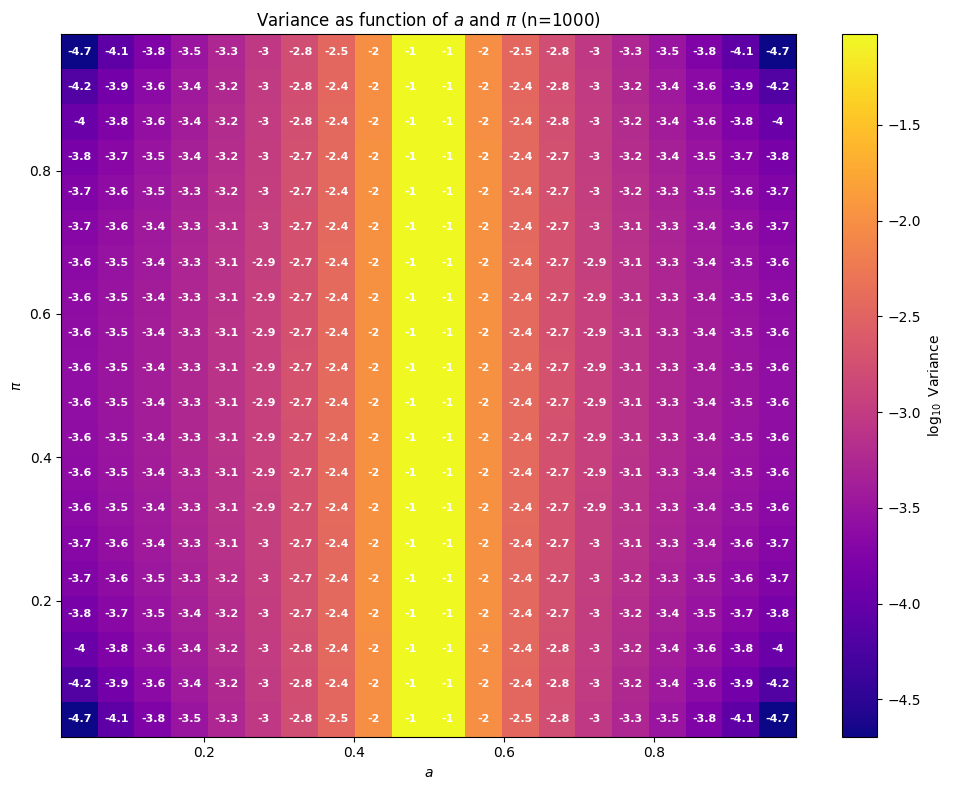
\includegraphics[width=\textwidth]{./heatmap.png}
    \caption{Variance of $\pi_{ML}$ as function of $a$ and $\pi$ for different values of $n$. Here, the values are log-scaled for better display. Note that we restrict $a\in [0.01, 0.99]$ and $\pi\in [0.01, 0.99]$ for the plot. Hence, very low values are expected whenever $a$ or $\pi$ exceeds these bounds.}
    \label{fig:variance_heatmap}
\end{figure}



\subsection{(g)}
\textit{Give an expression for the bias of this naive estimator. Is it asymptotically unbiased?}

We aim to recover the value of $\pi$ from direct questioning. 
However, persons belonging to the sensitive group will lie with probability $\ell$, whereas persons belonging to the non-sensitive group will answer truthfully and therefore lie with probability $0$.

Naivily, we could estimate the value of $\pi$ as the fraction of persons answering yes to the question:
\begin{equation*}
    \pi_\text{naive} = \frac{\sum_{i=1}^{n} X_i}{n}\;.
\end{equation*}

We can model the whether a person belongs to the sensitive group as a hidden variable $S_i \in \{0, 1\}$ with $S_i = 1$ describing that the person belongs to the sensitive group, and $S_i = 0$ describes that a person belongs to the non-sensitive group.

Naturally, we have that 
\begin{align*}
    P(S_i = 1) &= \pi \\
    P(S_i = 0) &= 1 - \pi
\end{align*}
which is distributed according to a Bernoulli distribution with parameter $p=\pi$.

We can now express the probability of a person answering yes or no to the question by marginalizing over the hidden variable $S_i$:
\begin{align*}
    P(X_i = 1) &= P(X_i = 1, S_i = 1) + P(X_i = 1, S_i = 0) \\
    &= \pi \cdot (1-\ell) + 0 \\
    P(X_i = 0) &= P(X_i = 0, S_i = 1) + P(X_i = 0, S_i = 0) \\
    &= \pi \cdot \ell + (1-\pi)\;.
\end{align*}

We verify that the probabilities are correct by adding both $P(X_i = 1)$ and $P(X_i = 0)$ and getting $1$:
\begin{align*}
    P(X_i = 1) + P(X_i = 0) &= \pi \cdot (1-\ell) + \pi \cdot \ell + (1-\pi) \\
    &= \pi (1-\ell + \ell) + 1- \pi \\
    &= \pi (1) + 1- \pi \\
    &= 1\;.
\end{align*}

We now compute the expeced value of the naive estimator of $\pi$ to check whether the estimator is unbiased.
We have
\begin{align*}
    \mathbb{E}[\pi_\text{naive}] &= \mathbb{E}\left[ \frac{\sum_{i=1}^{n} X_i}{n} \right] \\
    &= \frac{1}{n} \cdot \sum_{i=1}^{n} \mathbb{E}[X_i] \\
    &= \frac{1}{n} \cdot \sum_{i=1}^{n} \left( P(X_i = 1) \cdot 1 + P(X_i = 0) \cdot 0 \right) \\
    &= \frac{1}{n} \cdot \sum_{i=1}^{n} \left( P(X_i = 1) \right) \\
    &= \frac{1}{n} \cdot \sum_{i=1}^{n} \left( \pi \cdot (1-\ell) \right) \\
    &= \frac{1}{n} \cdot n \left( \pi \cdot (1-\ell) \right) \\
    &= \pi \cdot (1-\ell)\;. \stepandtag \label{eq:naive_expected_value}
\end{align*}

We can now use the expected value of $\pi_{\text{naive}}$ to compute the bias of the estimator:
\begin{align*}
    \text{Bias}(\pi_{\text{naive}}, \pi) &= {\left[ \mathbb{E}[\pi_{\text{naive}}] - \pi \right]}^2 \\
    &= {\left[ \pi \cdot (1-\ell) - \pi \right]}^2 \\
    &= {\left[ \pi - \pi \ell - \pi \right]}^2 \\
    &= {\left[ - \pi \ell \right]}^2 \\
    &= \pi^2 \ell^2\;. \stepandtag \label{eq:bias_naive}
\end{align*}

Therefore, only whenever $\ell = 0$, i.e., no one lies, is the naive estimator of $\pi$ is unbiased.
Otherwise, the estimator is biased towards and goes towards zero bias whenever either $\ell$ or $\pi$ goes to zero.


\subsection{(h)}
\textit{Derive expressions for the mean squared error (MSE) of the randomized response estimator and the naive estimator. Analyse the expressions to draw conclusions about when, depending on the relevant parameters $(\pi, a, \ell, n)$, one estimator should be favored over the other.}

We aim to compute the mean squared error of our two estimators of $\pi$.

% \begin{align*}
%     \text{MSE}(\pi_{\text{naive}}) &= \mathbb{E}\left[ {\left( \pi_{\text{naive}} - \pi \right)}^2 \right] \\
%     &= \mathbb{E} \left[ \pi_{\text{naive}}^2 + \pi^2 - 2\pi_{\text{naive}} \pi \right] \\
%     &= \mathbb{E} \left[ \pi_{\text{naive}}^2  \right] + \mathbb{E} \left[ \pi^2  \right] - \mathbb{E} \left[ 2\pi_{\text{naive}} \pi  \right] \\
%     &= \mathbb{E}\left[ {\left( \frac{\sum_{i=1}^{n} X_i}{n} \right)}^2 \right] + \pi^2 - 2 \pi \mathbb{E}\left[ \pi_{\text{naive}} \right] \\
%     &\overset{(\ref{eq:naive_expected_value})}{=} \mathbb{E}\left[ {\left( \frac{\sum_{i=1}^{n} X_i}{n} \right)}^2 \right] + \pi^2 - 2 \pi \left( \pi \cdot (1-\ell) \right) \\
%     &= \mathbb{E}\left[ {\left( \frac{\sum_{i=1}^{n} X_i}{n} \right)}^2 \right] + \pi^2 - 2 \pi^2 (1-\ell) \\
%     &= \mathbb{E}\left[ X_i \right]^2 + \pi^2 - 2 \pi^2 (1-\ell) \stepandtag \label{eq:mse_iid_assumption} \\
% \end{align*}
We use the Bias Variance decomposition to decompose the MSE into the bias and variance terms.\!\footnote{See \url{https://en.wikipedia.org/wiki/Mean_squared_error\#Proof_of_variance_and_bias_relationship}.}
Therefore, we simplify the MSE into 
\begin{align*}
    \text{MSE}(\hat{\pi}, \pi) &= \mathbb{E}\left[ {\left( \hat{\pi} - \mathbb{E}[\hat{\pi}] \right)}^2 \right] + {\left[ \mathbb{E}[\hat{\pi}] - \pi \right]}^2 \\
    &= \mathbb{V}\left[ \hat{\pi} \right] + {\left[ \mathbb{E}[\hat{\pi}] - \pi \right]}^2 \\
    &= \mathbb{V}\left[ \hat{\pi} \right] + \text{Bias}(\hat{\pi}, \pi) \\
\end{align*}
Therefore, we have
% \begin{align*}
%     \text{MSE}(\pi_{\text{naive}}, \pi) &= \mathbb{E}\left[ {\left( \mathbb{E}[\pi_{\text{naive}}] - \pi \right)}^2 \right] + {\left[ \mathbb{E}[\pi_{\text{naive}}] - \pi \right]}^2 \\
%     &= \mathbb{E}\left[ \mathbb{E}{[\pi_{\text{naive}}]}^2 + \pi^2 - 2\pi\mathbb{E}[\pi_{\text{naive}}]  \right] + {\left[ \mathbb{E}[\pi_{\text{naive}}] - \pi \right]}^2 \\
%     &= \mathbb{E}{[\pi_{\text{naive}}]}^2 + \mathbb{E}\left[ \pi^2  \right] - \mathbb{E}\left[ 2\pi\mathbb{E}[\pi_{\text{naive}}]  \right] + {\left[ \mathbb{E}[\pi_{\text{naive}}] - \pi \right]}^2 \\
%     &= \mathbb{E}{[\pi_{\text{naive}}]}^2 + \mathbb{E}\left[ \pi^2  \right] - 2\pi \mathbb{E}[\pi_{\text{naive}}] + {\left[ \mathbb{E}[\pi_{\text{naive}}] - \pi \right]}^2 \\
%     &\overset{(\ref{eq:naive_expected_value})}{=} {\left( \pi \cdot (1-\ell) \right)}^2 + \pi^2 - 2\pi \left( \pi \cdot (1-\ell) \right) + {\left[ \left( \pi \cdot (1-\ell) \right) - \pi \right]}^2 \\
%     &={\left( \pi \cdot (1-\ell) \right)}^2  + \pi^2 - 2\pi^2 \cdot (1-\ell) + {\left( \pi \cdot (1-\ell) \right)}^2 + \pi^2 - 2\pi\left( \pi \cdot (1-\ell) \right) \\
%     &= {\left( \pi \cdot (1-\ell) \right)}^2  + \pi^2 - 2\pi^2 \cdot (1-\ell) + {\left( \pi \cdot (1-\ell) \right)}^2 + \pi^2 - 2\pi^2 \cdot (1-\ell) \\
%     &= 2\pi^2 - 4\pi^2 \cdot (1-\ell) + 2{\left( \pi \cdot (1-\ell) \right)}^2  \\
%     &= 2\pi^2 - 4\pi^2 \cdot (1-\ell) + 2\pi^2 \cdot {(1-\ell)}^2  \\
%     &= 2\pi^2 \left( {(1-\ell)}^2 - 2(1-\ell) + 1 \right)  \\
%     &= 2\pi^2 \left( 1^2 + \ell^2 - 2\ell - 2 + 2\ell + 1 \right)  \\
%     &= 2\pi^2 \ell^2 
% \end{align*}
% Let us first compute $\mathbb{E}[\pi_\text{naive}^2]$ and ${\mathbb{E}[\pi_\text{naive}]}^2$.
% \begin{align*}
%     \mathbb{E}[\pi_\text{naive}^2] &= \mathbb{E} \left[ {\left( \frac{\sum_{i=1}^{n} X_i}{n} \right)}^2 \right] \\
%     &= \mathbb{E} \left[ {\left( \frac{\sum_{i=1}^{n} X_i}{n} \right)}^2 \right] \\
%     &= \mathbb{E} \left[ {\left( \frac{1}{n} \cdot \sum_{i=1}^{n} X_i \right)}^2 \right] \\
%     &= \mathbb{E} \left[ \frac{1}{n^2} {\left( \sum_{i=1}^{n} X_i \right)}^2 \right] \\
%     &= \frac{1}{n^2} \mathbb{E} \left[ {\left( \sum_{i=1}^{n} X_i \right)}^2 \right] \\
%     &= \frac{1}{n^2} \mathbb{E} \left[ n \cdot \mathbb{E}[X_i \cdot X_i] + (n^2 - n) \cdot \mathbb{E}[X_i \cdot X_j] \right] \\
%     &= \frac{1}{n^2} \mathbb{E} \left[ n \cdot \mathbb{E}[X_i^2] + (n^2 - n) \cdot \left( \mathbb{E}[X_i] + \mathbb{E}[X_j] \right) \right] \\
%     &= \frac{1}{n^2} \mathbb{E} \left[ n \cdot \mathbb{E}[X_i^2] + (n^2 - n) \cdot {\mathbb{E}[X_i]}^2 \right] \\
%     &= \frac{1}{n} \mathbb{E}[X_i^2] + \frac{n^2 - n}{n^2} \cdot {\mathbb{E}[X_i]}^2  \\
%     &= \frac{1}{n} \mathbb{E}[X_i^2] + \left( 1 - \frac{1}{n} \right) \cdot {\mathbb{E}[X_i]}^2  \\
%     &= \frac{1}{n} \mathbb{E}[X_i^2] + \left( \frac{n-1}{n} \right) \cdot {\mathbb{E}[X_i]}^2 \\
%     &= \frac{1}{n} \left[ P(X_i = 1) \cdot 1^2 + P(X_i = 0) \cdot 0^2 \right] + \left( \frac{n-1}{n}\right) \cdot {\left( P(X_i = 1) \cdot 1 + P(X_i = 0) \cdot 0 \right)}^2 \\
%     &= \frac{1}{n} \left[ P(X_i = 1)\right] + \left( \frac{n-1}{n} \right) \cdot {\left( P(X_i = 1) \right)}^2 \\
%     &= \frac{1}{n} \left[ \pi \cdot (1- \ell)\right] + \left( \frac{n-1}{n} \right) \cdot {\left( \pi \cdot (1- \ell) \right)}^2 \\
%     &= \frac{\pi \cdot (1- \ell)}{n} + \left( \frac{n-1}{n} \right) \cdot  \pi^2 \cdot {(1- \ell)}^2 
%     % &= \frac{1}{n} \left( \pi \cdot (1- \ell) + \left( n-1 \right) \cdot  \pi^2 \cdot {(1- \ell)}^2 \right) 
%     \stepandtag \label{eq:expectation_naive_x_i_square_outside} 
% \end{align*}

\begin{align*}
    \mathbb{V}[\pi_{\text{naive}}] &= \mathbb{V}\left[ \frac{\sum_{i=1}^{n} X_i}{n} \right] \\
    &= \frac{1}{n^2} \sum_{i=1}^{n} \mathbb{V}[X_i] \\
    &= \frac{1}{n^2} \sum_{i=1}^{n} \mathbb{E}[X_i^2] - {\mathbb{E}[X_i]}^2 \\
    &= \frac{1}{n^2} \sum_{i=1}^{n} \left[ P(X_i = 1) \right] - {\left( P(X_i = 1) \right)}^2 \\
    &= \frac{1}{n^2} \sum_{i=1}^{n} (\pi \cdot (1-\ell)) - {(\pi \cdot (1-\ell))}^2 \\
    &= \frac{n}{n^2} \left( (\pi \cdot (1-\ell)) - {(\pi \cdot (1-\ell))}^2 \right) \\
    &= \frac{\pi \cdot (1-\ell) - \pi^2 \cdot {(1-\ell)}^2}{n} \stepandtag \label{eq:variance_naive_x_i}
    % &= \frac{1}{n} \left( \pi \cdot (1-\ell) - \pi^2- \pi^2 \ell^2 \right) \\
\end{align*}

\begin{align*}
    \text{MSE}(\pi_{\text{naive}}, \pi) &= \mathbb{V}[\pi_{\text{naive}}] + \text{Bias}(\hat{\pi}, \pi) \\
    &\overset{(\ref{eq:variance_naive_x_i})}{=} \frac{\pi \cdot (1-\ell) - \pi^2 \cdot {(1-\ell)}^2}{n} + \text{Bias}(\hat{\pi}, \pi) \\
    &\overset{(\ref{eq:bias_naive})}{=} \frac{\pi \cdot (1-\ell) - \pi^2 \cdot {(1-\ell)}^2}{n} + \pi^2 \ell^2
    \;.
    % &= \frac{\pi \cdot (1-\ell) - \pi^2 \cdot {(1-\ell)}^2}{n} + {\mathbb{E}[\pi_{\text{naive}}]}^2 + \pi^2 - 2\pi \mathbb{E}\left[ \pi_{\text{naive}} \right] \\
    % &= \frac{\pi \cdot (1-\ell) - \pi^2 \cdot {(1-\ell)}^2}{n} + {\left( \pi \cdot (1-\ell) \right)}^2 + \pi^2 - 2\pi \pi \cdot (1-\ell) \\
    % &= \frac{\pi \cdot (1-\ell) - \pi^2 \cdot {(1-\ell)}^2}{n} + \pi^2 \cdot {(1-\ell)}^2 + \pi^2 - 2\pi^2 \cdot (1-\ell) \\
\end{align*}

Because the $\piml$ is an unbiased estimator of $\pi$, we have that $\text{Bias}(\piml, \pi) = 0$.
Therefore, we have
\begin{align*}
    \text{MSE}(\pi_{\text{ML}}, \pi) &= \mathbb{V}[\pi_{\text{ML}}] + \text{Bias}(\pi_{\text{ML}}, \pi) \\
    &= \mathbb{V}[\pi_{\text{ML}}] \\
    &\overset{(\ref{eq:variance_pi_ml})}{=} \frac{\pi - \pi^2}{n} + \frac{a - a^2}{{(2a-1)}^2 \cdot n}\;.
    % &\overset{(\ref{eq:variance_pi_ml})}{=} \frac{\pi - \pi^2}{n} + \frac{a - a^2}{(2^2a^2 +1^2 - 2a) \cdot n} \\
    % &\overset{(\ref{eq:variance_pi_ml})}{=} \frac{\pi - \pi^2}{n} - \frac{a - a^2}{2(a - \frac{1}{2} - 2a^2) \cdot n} \\
\end{align*}

First, we observe that whenever no-one lies ($\ell = 0$), the left side of the MSE of $\pi_{\text{naive}}$ is equal to the left side of the MSE of $\piml$. However, as the right side of the MSE of $\pi_{\text{naive}}$ is multiplied with $\ell^2$, the MSE is zero for $\ell = 0$, whereas the MSE of $\piml$ is non-zero, given $a\notin \{0, 1\}$. If $a\in \{0, 1\}$, then both estimators are equal w.r.t. the MSE.


% We now solve for both MSE expressions to be equal.
% \begin{align*}
%     \text{MSE}(\pi_{\text{naive}}, \pi) &= \text{MSE}(\pi_{\text{ML}}, \pi) \\
%     \frac{\pi \cdot (1-\ell) - \pi^2 \cdot {(1-\ell)}^2}{n} + \pi^2 \ell^2 & = \frac{\pi - \pi^2}{n} + \frac{a - a^2}{{(2a-1)}^2 \cdot n} &&\mid \cdot\  n \\
%     \pi \cdot (1-\ell) - \pi^2 \cdot {(1-\ell)}^2 + n \cdot \pi^2 \ell^2 & = \pi - \pi^2 + \frac{a - a^2}{{(2a-1)}^2} &&\mid \div \ \pi \\
%     (1-\ell) - \pi \cdot {(1-\ell)}^2 + n \cdot \pi \ell^2 & = 1 - \pi + \frac{a - a^2}{{(2a-1)}^2 \cdot \pi}  \stepandtag \label{eq:mse_equal} \;.
% \end{align*}

% First, we observe that Equation~\ref{eq:mse_equal} for the MSE of $\pi_{\text{naive}}$ increases w.r.t. $n$ whenever $\ell > 0$ and $\pi > 0$, whereas the MSE of $\piml$ does not depend on $n$.
% Therefore, this shows that with increasing sample size, the MSE of $\piml$ decreases faster than the MSE for $\pi_{\text{naive}}$. Therefore, for large sample size, $\piml$ should be preferred over $\pi_{\text{naive}}$.

Due to the complex expressions, finding the cut-off points for when both MSE expressions are equal --- and therefore finding whenever one estimator is better than the other analytically --- is very complicated.
While we have explained the trivial edge cases, whenever we have $a \notin \{0, 1\} \land \pi \notin \{0, 1\}$, we have no easy way to determine when which estimator is better than the other. To overcome this issue, we have computed the expected MSE for both estimators for a range of values for $a, \pi, \ell$, and $n$ and show the results in Figure~\ref{fig:mse_naive_better}. 
Figure~\ref{fig:mse_naive_better} clearly shows the complex, non-linear relationship between both MSE expression. 

First, it is clear that no single best estimator exists for all parameters. 
The shape of the region where $\pi_{naive}$ has a lower MSE than $\piml$ is quite clear:
whenever $\ell = 0$, the naive estimator is better than the ML estimator. Furthermore, whenever $\pi = 0$, the naive estimator is also better. Both cases make sense, as whenever no one lies, the naive estimator is the better estimator of the two.


\begin{figure}[htbp]
    \centering
    % 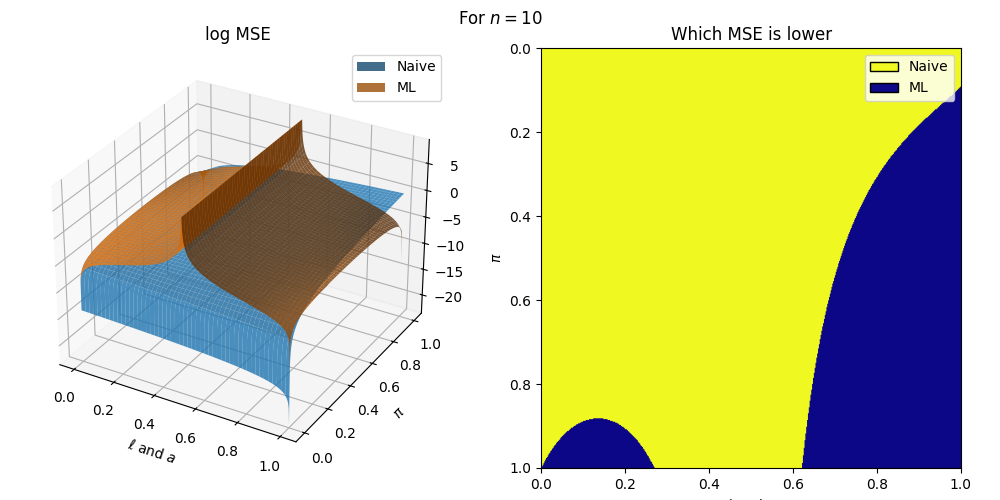
\includegraphics[width=0.7\textwidth]{MSE_naive_vs_ml_10.png}
    % 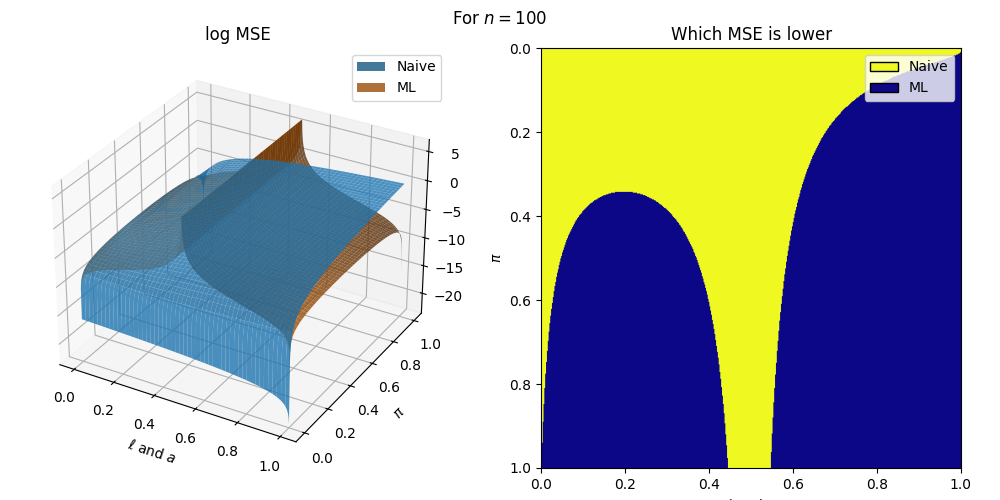
\includegraphics[width=0.7\textwidth]{MSE_naive_vs_ml_100.png}
    \subfloat[For $n = 10$]{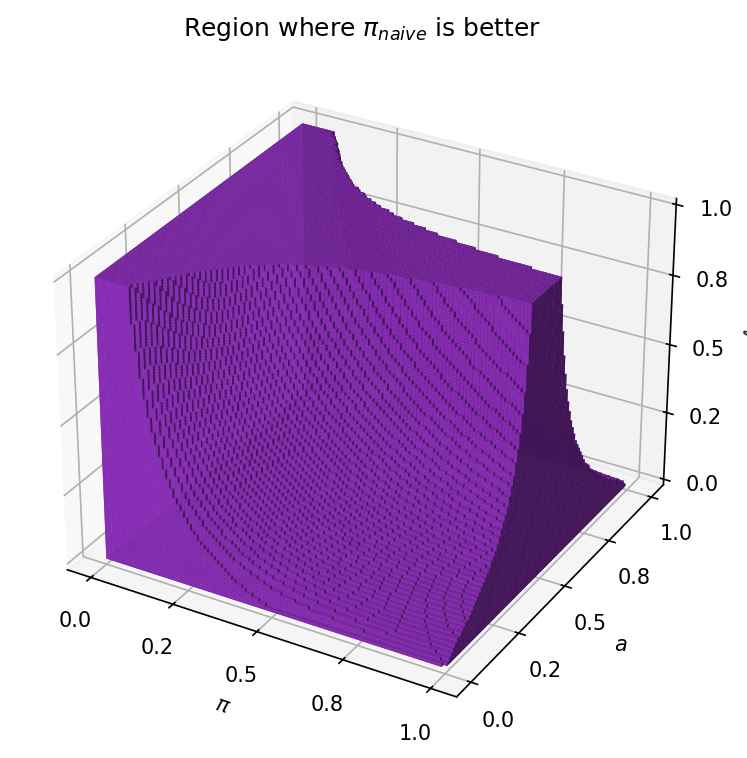
\includegraphics[width = 2.5in]{rregion_10.png}}
    % \subcaption{Meow}
    \subfloat[For $n = 100$]{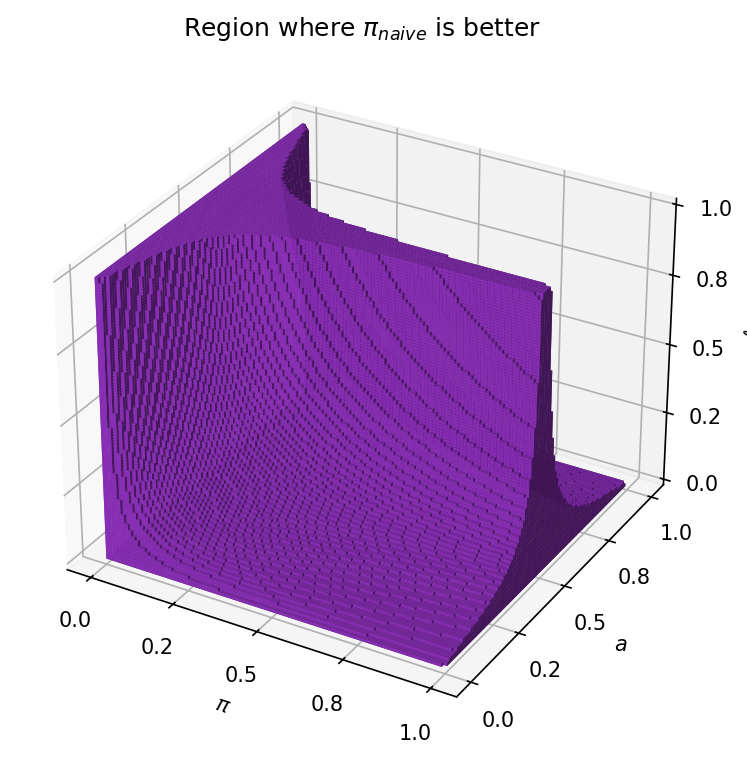
\includegraphics[width = 2.5in]{rregion_100.png}}\\
    \subfloat[For $n = 1\ 000$]{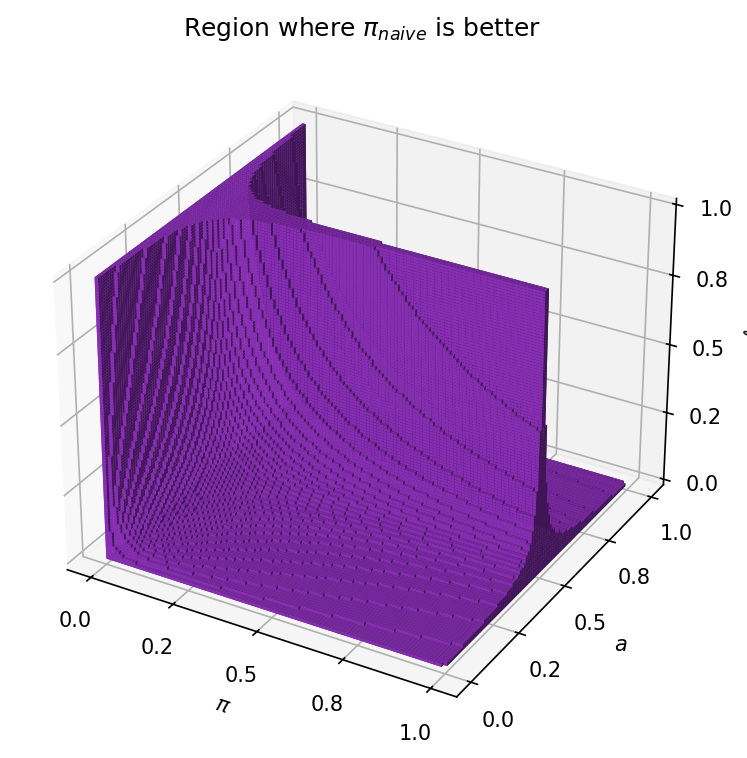
\includegraphics[width = 2.5in]{rregion_1000.png}}
    \subfloat[For $n = 10\ 000$]{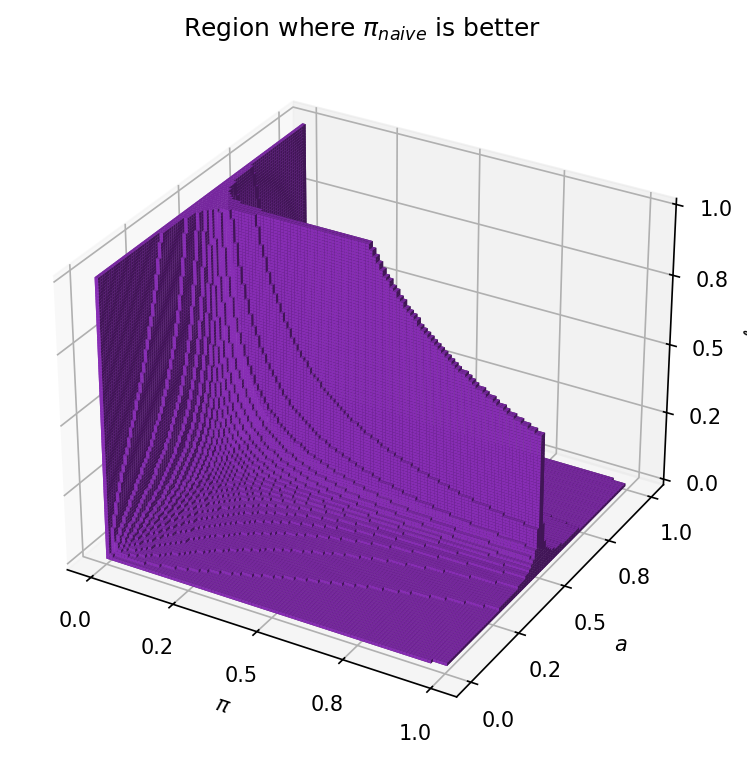
\includegraphics[width = 2.5in]{rregion_10000.png}} 
    \caption{Plots of the parameter space of $(\pi, a, \ell)$ for various sample sizes $n$. The purple voxels indicate for which parameters the MSE of $\pi_{naive}$ is lower than the MSE of $\piml$. Note that plot is mirrored around the $\ell$-axis at $a = 0.5$.}
    % \caption{In each subfigure, we plot the MSE of $\piml$ and $\pi_{\text{naive}}$ in 3D (left) and indicate with what parameters the MSE of $$}
    \label{fig:mse_naive_better}
\end{figure}

Figure~\ref{fig:mse_naive_better} also shows that whenever $a$ is close or equal to $0.5$, the naive estimator is the better solution. Note that while our plot shows that in the subplot (d), for some parameters which include $a=0.5$, the ML estimator is to be favored. This is not true, as it is simply an artefact of the plotting; We use only 100 points for each axis, and therefore the voxels are quite large. With increased resolution, the same plot would show that the naive estimator is the better solution for these parameters.

Lastly, for all other cases that we did not mention, the ML estimator is the better solution for large $n$. Refer to Figure~\ref{fig:mse_naive_better} for the exact shape. This is logical, as the MSE of the naive estimator has a part independent of $n$, whereas the MSE of the ML estimator is entirely divided by $n$. Thus, for large $n$, the ML estimator will go towards zero, whereas the naive estimator will remain constant.

% While Figure~\ref{} clearly shows the complex, non-linear relationship between both MSE expression, we vary the values of $a$ and $\ell$ together. This only shows a slice of the full parameter space. Therefore, we also plot the region where $\pi_{\text{naive}}$ has a lower MSE than $\piml$ in Figure~\ref{} when varying $\pi, a$, and $\ell$ independently.


% \begin{figure}[h]
%     \centering
%     % 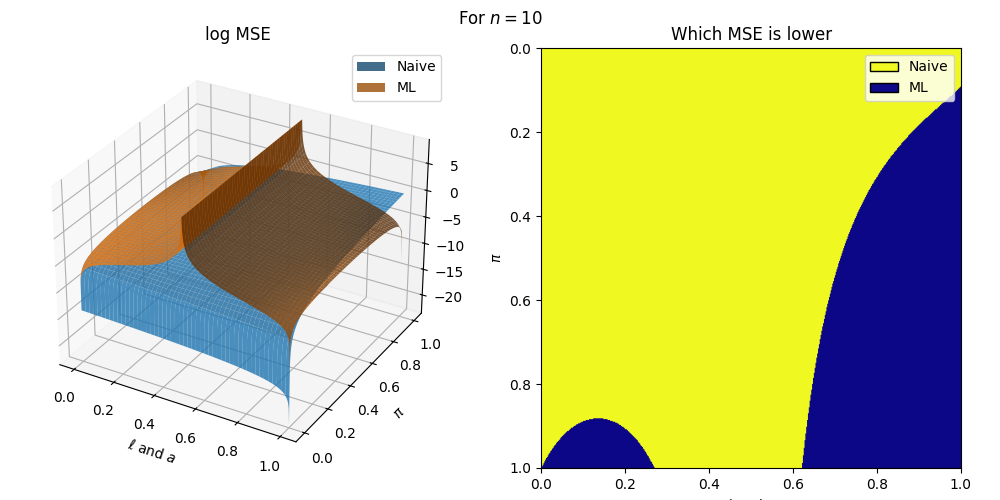
\includegraphics[width=0.7\textwidth]{MSE_naive_vs_ml_10.png}
%     % 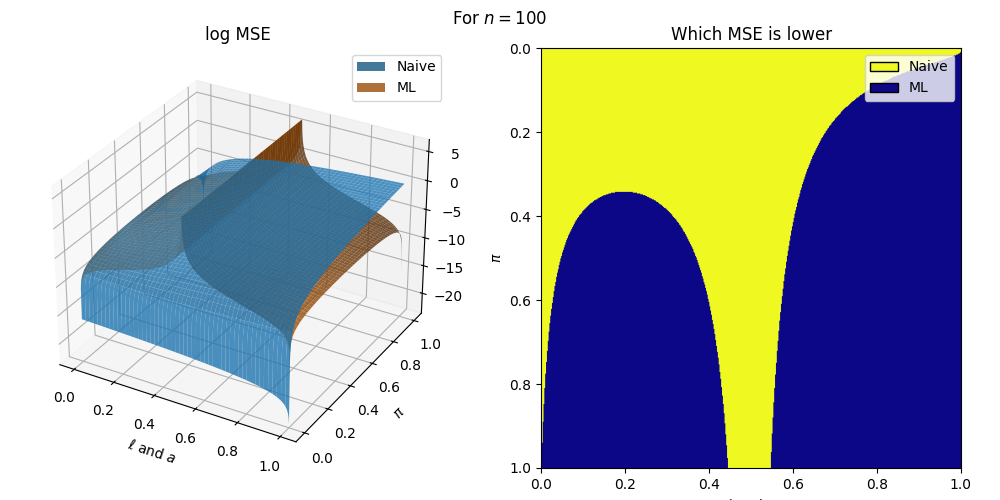
\includegraphics[width=0.7\textwidth]{MSE_naive_vs_ml_100.png}
%     \subfloat[For $n = 10$]{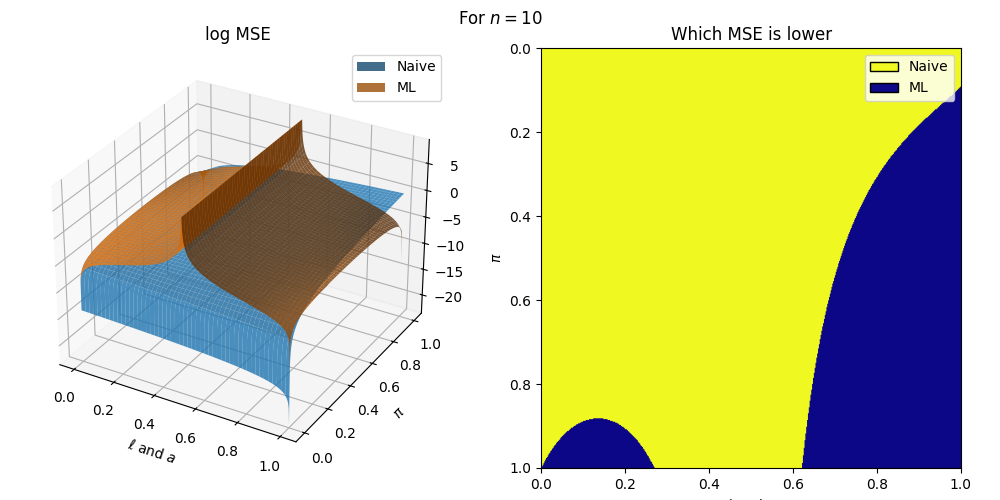
\includegraphics[width = 3in]{MSE_naive_vs_ml_10.png}}
%     % \subcaption{Meow}
%     \subfloat[For $n = 100$]{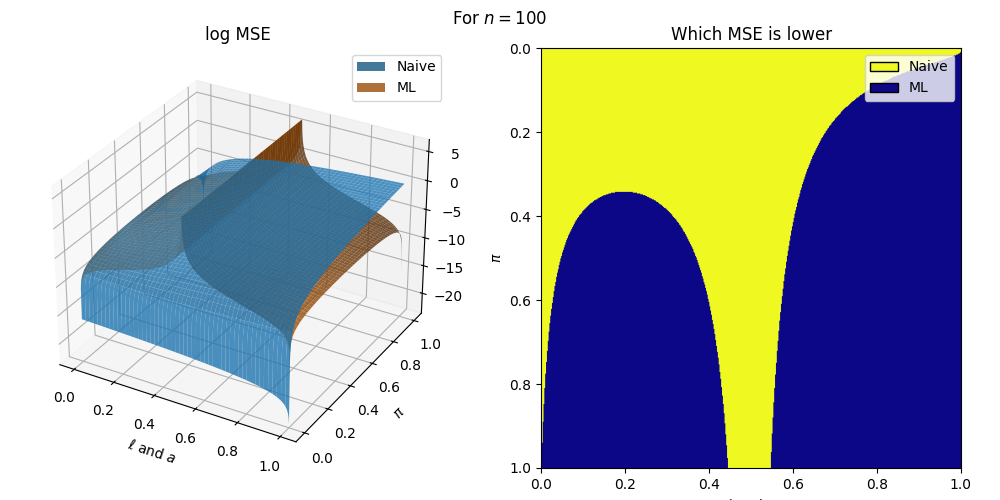
\includegraphics[width = 3in]{MSE_naive_vs_ml_100.png}}\\
%     \subfloat[For $n = 1\ 000$]{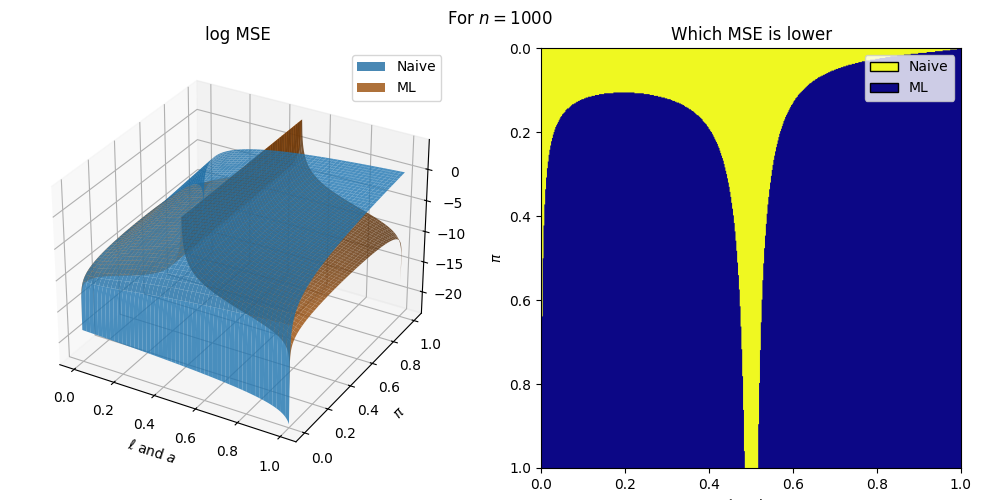
\includegraphics[width = 3in]{MSE_naive_vs_ml_1000.png}}
%     \subfloat[For $n = 10\ 000$]{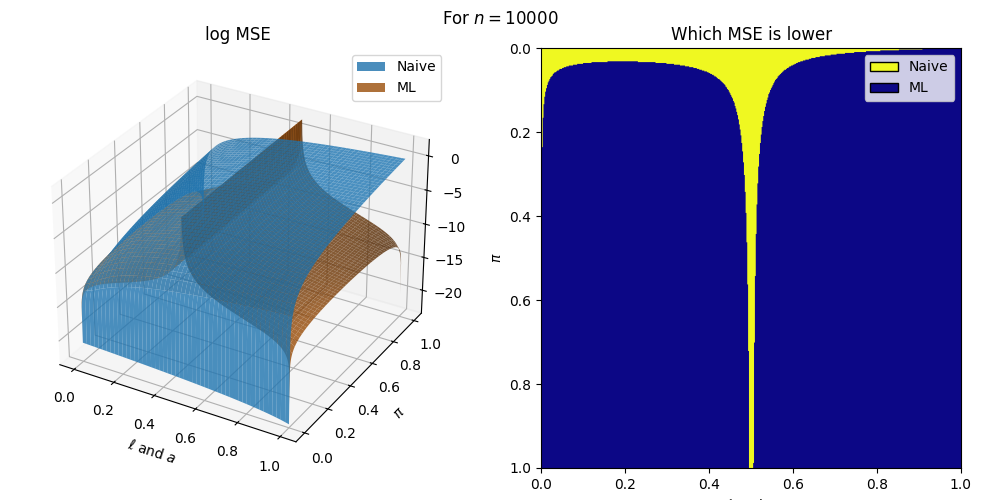
\includegraphics[width = 3in]{MSE_naive_vs_ml_10000.png}} 
%     \caption{\textbf{Left}: log MSE of $\piml$ and $\pi_{\text{naive}}$ in 3D. \textbf{Right}: The region indicating whenever an estimator has a lower MSE than the other. In this figure, we link $a$ and $\ell$ together (they are both on the same axis) as the MSE for both estimators depends on only one of them.}
%     % \caption{In each subfigure, we plot the MSE of $\piml$ and $\pi_{\text{naive}}$ in 3D (left) and indicate with what parameters the MSE of $$}
%     \label{fig:mse_naive_vs_ml}
% \end{figure}



% Let us now analyze the critical points of both MSE expressions, i.e., whenever they are both equal, to determine when one estimator has a lower MSE than the other.

% Let us first solve for $\ell$:
% \begin{align*}
%     \text{MSE}(\pi_{\text{naive}}, \pi) &= \text{MSE}(\pi_{\text{ML}}, \pi) \\
%     \frac{\pi \cdot (1-\ell) - \pi^2 \cdot {(1-\ell)}^2}{n} + \pi^2 \ell^2 &= \frac{\pi - \pi^2}{n} + \frac{a - a^2}{{(2a-1)}^2 \cdot n} \\
%     \frac{\pi \cdot (1-\ell) - \pi^2 \cdot {(1-\ell)}^2}{n} &= \frac{\pi - \pi^2}{n} + \frac{a - a^2}{{(2a-1)}^2 \cdot n} -  \pi^2 \ell^2 \\
%     \pi \cdot (1-\ell) - \pi^2 \cdot {(1-\ell)}^2 &= \pi - \pi^ 2+ \frac{a - a^2}{{(2a-1)}^2} -  n\cdot\pi^2 \ell^2 \\ 
%     \pi - \ell \pi - \pi^2 \cdot \left( 1 + \ell^2 - 2\ell \right) &= \pi - \pi^ 2+ \frac{a - a^2}{{(2a-1)}^2} -  n\cdot\pi^2 \ell^2 &&\mid \div\ \pi \\ 
%     1 - \ell - \pi \cdot \left( 1 + \ell^2 - 2\ell \right) &= 1 - \pi + \frac{a - a^2}{{(2a-1)}^2\cdot\pi} -  n\cdot\pi \ell^2 \\ 
%     \ell + \pi\ell^2 + 2\ell \pi + n\cdot\pi \ell^2  &= \frac{a - a^2}{{(2a-1)}^2\cdot\pi}  \\ 
%     \ell \left( 1 + 2 \pi \right) + \ell^2 \left( \pi + n \cdot \pi \right)  &= \frac{a - a^2}{{(2a-1)}^2\cdot\pi}  \\ 
%     \ell \frac{\left( 1 + 2 \pi \right)}{\left( \pi + n \cdot \pi \right)}  + \ell^2  &= \frac{a - a^2}{{(2a-1)}^2\cdot\pi \cdot \left( \pi + n \cdot \pi \right)}  \\ 
%     \ell^2 + \ell \frac{\left( 1 + 2 \pi \right)}{\left( \pi + n \cdot \pi \right)} - \frac{a - a^2}{{(2a-1)}^2\cdot\pi \cdot \left( \pi + n \cdot \pi \right)}  &= 0  \\ 
%     \ell^2 + \ell \frac{\left( 1 + 2 \pi \right)}{\pi\left( n+1 \right)} - \frac{a - a^2}{{(2a-1)}^2\cdot\pi^2 \cdot \left( n+1 \right)}  &= 0  \\ 
% \end{align*}
% where the equation trivialy holds for the following points:
% \begin{itemize}
%     \item $\ell = 0, a = 1, \pi\neq 0$
%     \item $\ell = 0, a = 0, \pi \neq 0$
%     \item $\ell = 0, n=\infty, a\neq 0.5, \pi \neq 0$
% \end{itemize}
% however, for points, we need to solve the quadratic equation. To this end, we use the quadratic formula.
% We set 
% \begin{equation*}
%     p = \frac{\left( 1 + 2 \pi \right)}{\left( \pi + n \cdot \pi \right)} \\
% \end{equation*}
% and 
% \begin{equation*}
%     q = - \frac{a - a^2}{{(2a-1)}^2\cdot\pi^2 \cdot \left( n+1 \right)}\;.
% \end{equation*}
% We therefore have
% \begin{align*}
%     \ell_1, \ell_2 &= - \frac{p}{2} \pm \sqrt{{\left( \frac{p}{2} \right)}^2 - q} \\
%     &= -\frac{ 1 + 2 \pi }{2 \left( \pi + n \cdot \pi \right)} \pm \sqrt{\frac{{\left( 1 + 2 \pi \right)}^2}{{2\left( \pi + n \cdot \pi \right)}^2} + \frac{a - a^2}{{(2a-1)}^2\cdot\pi^2 \cdot \left( n+1 \right)}} \\
%     % &= -\frac{ 1 + 2 \pi }{2 \left( \pi + n \cdot \pi \right)} \pm \sqrt{\frac{{\left( 1 + 2 \pi \right)}^2}{{2\left( \pi + n \cdot \pi \right)}^2} + \frac{a - a^2}{\left( 2^2a^2+1 - 2a \right)\cdot\pi^2 \cdot \left( n+1 \right)}} \\
% \end{align*}

% \begin{align*}
%     \text{MSE}(\pi_{\text{naive}}, \pi) &= \mathbb{E}\left[ {\left( \pi_{\text{naive}} - \mathbb{E}[\pi_{\text{naive}}] \right)}^2 \right] + {\left[ \mathbb{E}[\pi_{\text{naive}}] - \pi_{\text{naive}} \right]}^2 \\
%     &= \mathbb{E}\left[ \mathbb{E}{[\pi_{\text{naive}}]}^2 + \pi_{\text{naive}}^2 - 2\pi_{\text{naive}}\mathbb{E}[\pi_{\text{naive}}]  \right] + {\left[ \mathbb{E}[\pi_{\text{naive}}] - \pi \right]}^2 \\
%     &= \mathbb{E}{[\pi_{\text{naive}}]}^2 + \mathbb{E}\left[ \pi_{\text{naive}}^2  \right] -   2\pi_{\text{naive}}\mathbb{E}[\pi_{\text{naive}}] + \mathbb{E}{[\pi_{\text{naive}}]}^2 + \pi^2 - 2\pi  \mathbb{E}[\pi_{\text{naive}}] \\
%     % &= 2\mathbb{E}{[\pi_{\text{naive}}]}^2 + \mathbb{E}\left[ \pi_{\text{naive}}^2  \right] + \pi^2 - 4\pi  \mathbb{E}[\pi_{\text{naive}}] \\
%     &= 2\mathbb{E}{[\pi_{\text{naive}}]}^2 + \mathbb{E}\left[ \pi_{\text{naive}}^2  \right] + \pi^2 + \mathbb{E}[\pi_{\text{naive}}]\cdot(2\pi - 2 \pi_{\text{naive}}) \\
%     % &=  2\mathbb{E}{[\pi_{\text{naive}}]}^2 + \mathbb{E}\left[ \pi_{\text{naive}}^2  \right] + \pi^2 + \mathbb{E}[\pi_{\text{naive}}]\cdot(2\pi - 2 \pi_{\text{naive}}) \\
%     &\overset{(\ref{eq:expectation_naive_x_i_square_outside})}{=}  2\mathbb{E}{[\pi_{\text{naive}}]}^2 + \frac{\pi \cdot (1- \ell)}{n} + \left( \frac{n-1}{n} \right) \cdot  \pi^2 \cdot {(1- \ell)}^2 + \pi^2 - \mathbb{E}[\pi_{\text{naive}}]\cdot(2\pi + 2 \pi_{\text{naive}}) \\
%     % &\overset{(\ref{eq:expectation_naive_x_i_square_outside})}{=} 2\mathbb{E}{[\pi_{\text{naive}}]}^2 + \frac{\pi \cdot (1- \ell)}{n} + \left( \frac{n-1}{n} \right) \cdot  \pi^2 \cdot {(1- \ell)}^2 + \\
%     &\overset{(\ref{eq:naive_expected_value})}{=} 2 {\left[ \pi \cdot (1-\ell) \right]}^2 + \frac{\pi \cdot (1- \ell)}{n} + \left( \frac{n-1}{n} \right) \cdot  \pi^2 \cdot {(1- \ell)}^2 + \pi^2 -\left( \pi \cdot (1-\ell) \right)\cdot(2\pi + 2 \pi_{\text{naive}}) \\
%     &\overset{(\ref{eq:naive_expected_value})}{=} 2 {\left[ \pi \cdot (1-\ell) \right]}^2 + \frac{\pi \cdot (1- \ell)}{n} + \left( \frac{n-1}{n} \right) \cdot  \pi^2 \cdot {(1- \ell)}^2 + \pi^2 - \left( \pi \cdot (1-\ell) \right)\cdot(2\pi + 2 \pi_{\text{naive}}) \\
%     &= 2 {\left[ \pi \cdot (1-\ell) \right]}^2 + \frac{\pi \cdot (1- \ell)}{n} + \left( \frac{n-1}{n} \right) \cdot  \pi^2 \cdot {(1- \ell)}^2 + \pi^2 - 2\pi \cdot (1-\ell) \cdot(\pi +  \pi_{\text{naive}}) \\
%     &= 2 \pi^2 \cdot {(1-\ell)}^2 + \frac{\pi \cdot (1- \ell)}{n} + \left( \frac{n-1}{n} \right) \cdot  \pi^2 \cdot {(1- \ell)}^2 + \pi^2 - 2\pi \cdot (1-\ell) \cdot(\pi +  \pi_{\text{naive}}) \\
%     &= \left( 1-\ell \right) \cdot \left( 2\pi^2 \cdot (1-\ell) + \frac{\pi}{n} + \left( \frac{n-1}{n} \right) \cdot  \pi^2 \cdot {(1- \ell)} - 2\pi (\pi +  \pi_{\text{naive}}) \right) \\
%     &= \left( 1-\ell \right) \cdot \left( 2\pi^2 \cdot (1-\ell) + \frac{\pi}{n} + \left( \frac{n-1}{n} \right) \cdot  \pi^2 \cdot {(1- \ell)} - 2\pi^2 -  2\pi\pi_{\text{naive}} \right) \\
%     &= \pi \cdot \left( 1-\ell \right) \cdot \left( 2\pi \cdot (1-\ell) + \frac{1}{n} + \left( \frac{n-1}{n} \right) \cdot  \pi \cdot {(1- \ell)} - 2\pi -  2\pi_{\text{naive}} \right) \\
%     &= \pi \cdot \left( 1-\ell \right) \cdot \left( 2\pi -2\pi \ell + \frac{1}{n} + \left( \frac{n-1}{n} \right) \cdot  \pi \cdot {(1- \ell)} - 2\pi -  2\pi_{\text{naive}} \right) \\
%     % &= 2 \pi^2 \cdot {(1-\ell)}^2 + \frac{\pi \cdot (1- \ell)}{n} + \left( \frac{n-1}{n} \right) \cdot  \pi^2 \cdot {(1- \ell)}^2 + \pi^2 + 2 \pi^2 \cdot (1-\ell) - 2 \pi_{\text{naive}} \pi \cdot (1-\ell) \\
%     % &= \pi^2 \left( 2 \cdot {(1-\ell)}^2 + \left( \frac{n-1}{n} \right)\cdot {(1-\ell)}^2 + 1 + 2 \cdot (1-\ell)  \right) + \frac{\pi \cdot (1- \ell)}{n} - 2 \pi_{\text{naive}} \pi \cdot (1-\ell) \\
%     % &= \pi^2 \left( 2- 2\ell^2 + \left( \frac{n-1}{n} \right) - \left( \frac{(n-1) \ell}{n} \right) + 1 + 2-2\ell  \right) + \frac{\pi \cdot (1- \ell)}{n} - 2 \pi_{\text{naive}} \pi \cdot (1-\ell) \\
%     % &= \pi^2 \left( 5- 2\ell^2 + \left( \frac{n-1}{n} \right) - \left( \frac{(n-1) \ell}{n} \right) -2\ell  \right) + \frac{\pi \cdot (1- \ell)}{n} - 2 \pi_{\text{naive}} \pi \cdot (1-\ell) \\
%     % % &= 2 \pi^2 \cdot {(1-\ell)}^2 + \frac{\pi \cdot (1- \ell)}{n} + \left( \frac{n-1}{n} \right) \cdot  \pi^2 \cdot {(1- \ell)}^2 + \pi^2 - 4\pi^2 \cdot (1-\ell) \\
% \end{align*}

% \pagebreak
% We have
% \todo[inline]{This is for the non-naive estimator.}
% \begin{align*}
%     \text{MSE}(\pi_\text{naive}) &= \mathbb{E}\left[ {(\pi_\text{naive} - \pi)}^2 \right] \\
%     &= \mathbb{E} \left[ {\left( \frac{\sum_{i=1}^{n} X_i}{n} - \pi \right)}^2 \right] \\
%     &= \mathbb{E} \left[ \frac{\sum_{i=1}^{n} X_i^2}{n^2} + \pi^2 - 2\pi\frac{\sum_{i=1}^{n} X_i}{n}  \right] \\
%     &= \mathbb{E} \left[ \frac{\sum_{i=1}^{n} X_i^2}{n^2} \right] + \mathbb{E} \left[ \pi^2 \right] - \mathbb{E} \left[ 2\pi\frac{\sum_{i=1}^{n} X_i}{n} \right] \\
%     &= \frac{1}{n^2} \sum_{i=1}^{n} \mathbb{E} \left[ X_i^2 \right] + \pi^2 - \frac{2 \pi}{n} \sum_{i=1}^{n} \mathbb{E}[X_i] \\
%     &\overset{(\ref{eq:expectation_naive_x_i_square_inside})}{=} \frac{1}{n^2} \sum_{i=1}^{n} \left[ (1-a) + (2a - 1) \cdot \pi \right] + \pi^2 - \frac{2 \pi}{n} \sum_{i=1}^{n} \mathbb{E}[X_i] \\
%     &= \frac{1}{n} \left[ (1-a) + (2a - 1) \cdot \pi \right] + \pi^2 - \frac{2 \pi}{n} \sum_{i=1}^{n} \mathbb{E}[X_i] \\
%     &\overset{(\ref{eq:expectation_naive_x_i_square_outside})}{=} \frac{1}{n} \left[ (1-a) + (2a - 1) \cdot \pi \right] + \pi^2 - \frac{2 \pi}{n} \sum_{i=1}^{n} \left[ 1 + \pi \left(6a - 4a^2 - 2 \right) + \pi^2 (4 a^2 - 4 a + 1) - 2a + a^2 \right] \\
%     &= \frac{1}{n} \left[ (1-a) + (2a - 1) \cdot \pi \right] + \pi^2 - 2 \pi \cdot \left[ 1 + \pi \left(6a - 4a^2 - 2 \right) + \pi^2 (4 a^2 - 4 a + 1) - 2a + a^2 \right] \\
%     &= \frac{(1-a)}{n} + \frac{(2a - 1) \cdot \pi }{n}
%      + \pi^2 - 2 \pi 
%     - 2 \pi^2 \left(6a - 4a^2 - 2 \right) - 2 \pi^3 (4 a^2 - 4 a + 1) + 4 \pi a - 2 \pi a^2  \\
%     &= \pi \left( \frac{2a -1}{n} - 2 + 4a - 2a^2 \right) + \pi^2 (1 - 12a + 4a^2 - 4) + \pi^3 ()
% \end{align*}


\pagebreak
\section{Problem 2}


We have implemented the given formulas for estimating the population size $\hat{N}$ and its variance $\hat{\sigma}_{\hat{N}}$ given some probability distributions from which we sample the probability of catching one animal. 
We have run the Monte-Carlo simulations for 1000 runs for each given probabiliy distribution and report on the computed values in Table~\ref{tab:problem_2_results_uniform_0_01} for $p_i \sim U(0, 0.01)$, Table~\ref{tab:problem_2_results_uniform_0_02} for $p_i \sim U(0, 0.02)$, Table~\ref{tab:problem_2_results_beta_1_3} for $p_i \sim 0.02 \cdot \mathrm{Beta}(1, 3)$, and Table~\ref{tab:problem_2_results_beta_2_2} for $p_i \sim 0.01 \cdot \mathrm{Beta}(2, 2)$.

Note that for the sake of ease of comparison, we report on $\hat{\sigma}_{\hat{N}} = \sqrt{\hat{\sigma}_{\hat{N}}^2}$ instead of the variance $\hat{\sigma}_{\hat{N}}^2$ as it allows us to directly compare it with the reported standard deviations of the other parameters.

% \todo[inline]{Compute expected value of catching one animal by 
% $\mathbb{E}[\Pr(X_i^t = 1)] = \int_0^1 Pr(p \leq q) dq\quad p \sim \Pr(\cdot) \Leftrightarrow \int_0^1 \int_0^q Pr(p' = p) dp' dq$ (something around double integral...)}

In this question, we are interested in the differences that arise from the different probability distributions, besides their performances. 
% Therefore, we will set out focus on their comparisons.

We first plot the probability distribution for the four probability distributions that we are investigating in Figure~\ref{fig:probability_density_functions}. From that figure, we hypothesize that the expected value of catching one animal is not the same for all four probability distributions. Therefore, let us first compute the expected value of catching one animal for each probability distribution. 

For the uniform distribution $U(0, a)$, with $a\in \mathbb{R}\setminus \{0\}$, we have:
\begin{align*}
    \mathbb{E}_{p \sim U(0, a)}[X_i^t] &= \mathbb{E}_{p \sim U(0, a), q\sim U(0, 1)}\left[ q \leq p \right] \\
    &= \mathbb{E}_{p \sim U(0, a)}\left[ \mathbb{E}_{q\sim U(0, 1)} \left[ q \leq p \right] \right] \\
    &= \int_0^a f_p(p) \cdot \mathbb{E}_{q\sim U(0, 1)} \left[ q \leq p \right] \  dp \\ 
    &= \int_0^a \frac{1}{a} \cdot \mathbb{E}_{q\sim U(0, 1)} \left[ q \leq p \right] \  dp \\ 
    &= \frac{1}{a} \int_0^a \mathbb{E}_{q\sim U(0, 1)} \left[ q \leq p \right] \  dp \\ 
    &= \frac{1}{a} \int_0^a \int_0^1 f_q(q) \cdot \mathbb{1}\{q \leq p\} \ dq \  dp \\
    &= \frac{1}{a} \int_0^a \int_0^1 1 \cdot \mathbb{1}\{q \leq p\} \ dq \  dp \\
    % &= \frac{1}{a} \int_0^a \int_0^1 \mathbb{1}\{q \leq p\} \ dq \  dp \\
    &= \frac{1}{a} \int_0^a \int_0^p 1 \ dq \  dp \\
    &= \frac{1}{a} \int_0^a {\left[ q \right]}_0^p \  dp \\
    &= \frac{1}{a} \int_0^a p \  dp \\
    &= \frac{1}{a} {\left[ \frac{p^2}{2} \right]}_0^a \\
    &= \frac{1}{a} \frac{a^2}{2} \\
    &= \frac{a}{2} \;.
\end{align*}

It naturally follows that 
\begin{equation}
    \mathbb{E}_{p \sim U(0, 0.01)}[X_i^t] = 0.005
    \label{eq:expectation_xi_u01}
\end{equation}
and
\begin{equation}
    \mathbb{E}_{p \sim U(0, 0.02)}[X_i^t] = 0.01\;.
    \label{eq:expectation_xi_u02}
\end{equation}

For $p\sim \mathrm{Beta}(\cdot)$, we have:
\begin{align*}
    \mathbb{E}_{p \sim \mathrm{Beta}(\alpha, \beta)}[X_i^t] &= \mathbb{E}_{p \sim \mathrm{Beta}(\alpha, \beta), q\sim U(0, 1)}\left[ q \leq p \right] \\
    &= \mathbb{E}_{p \sim \mathrm{Beta}(\alpha, \beta)}\left[ \mathbb{E}_{q\sim U(0, 1)} \left[ q \leq p \right] \right] \\
    &= \int_0^1 f_{\mathrm{Beta}(\alpha, \beta)}(p) \cdot \mathbb{E}_{q\sim U(0, 1)} \left[ q \leq p \right]\ dp\\
    &= \int_0^1 f_{\mathrm{Beta}(\alpha, \beta)}(p) \cdot \int_0^1 f_q(q) \cdot \mathbb{1}\{q \leq p\} \ dq \ dp\\
    &= \int_0^1 f_{\mathrm{Beta}(\alpha, \beta)}(p) \cdot p \  dp \\
    &= \mathbb{E}_{X\sim \mathrm{Beta}(\alpha, \beta)}\left[ X \right] \\
    &= \frac{\alpha}{\alpha + \beta}\;. 
    \stepandtag \label{eq:expectation_beta}
\end{align*}
Note that if $p\sim a \cdot \mathrm{Beta}(\cdot)$ with $a\in \mathbb{R} \setminus \{0\}$, we can just multiply Equation~\ref{eq:expectation_beta} with $a$ due to the properties of the expectation and the integrals. $a$ would be contained in the density function as a multiplicative factor, and thus, we can extract it.
Note that I got the expectation of the Beta distribution from wikipedia.\!\footnote{\url{https://en.wikipedia.org/wiki/Beta_distribution}}

Therefore, it follows that 
\begin{equation}
    \mathbb{E}_{p \sim 0.02 \cdot \mathrm{Beta}(1, 3)}[X_i^t] = 0.02 \cdot \frac{1}{4} = 0.005
    \label{eq:expectation_xi_beta13}
\end{equation}
and 
\begin{equation}
    \mathbb{E}_{p \sim 0.01 \cdot \mathrm{Beta}(2, 2)}[X_i^t] = 0.01 \cdot \frac{1}{2} = 0.005\;.
    \label{eq:expectation_xi_beta22}
\end{equation}

The usefulness of Equation~\ref{eq:expectation_xi_u01}--\ref{eq:expectation_xi_u02} and Equation~\ref{eq:expectation_xi_beta13}--{\ref{eq:expectation_xi_beta22}} expected values will become clear in the next section.

\vspace{1em}

\begin{figure}[t]
    \centering
    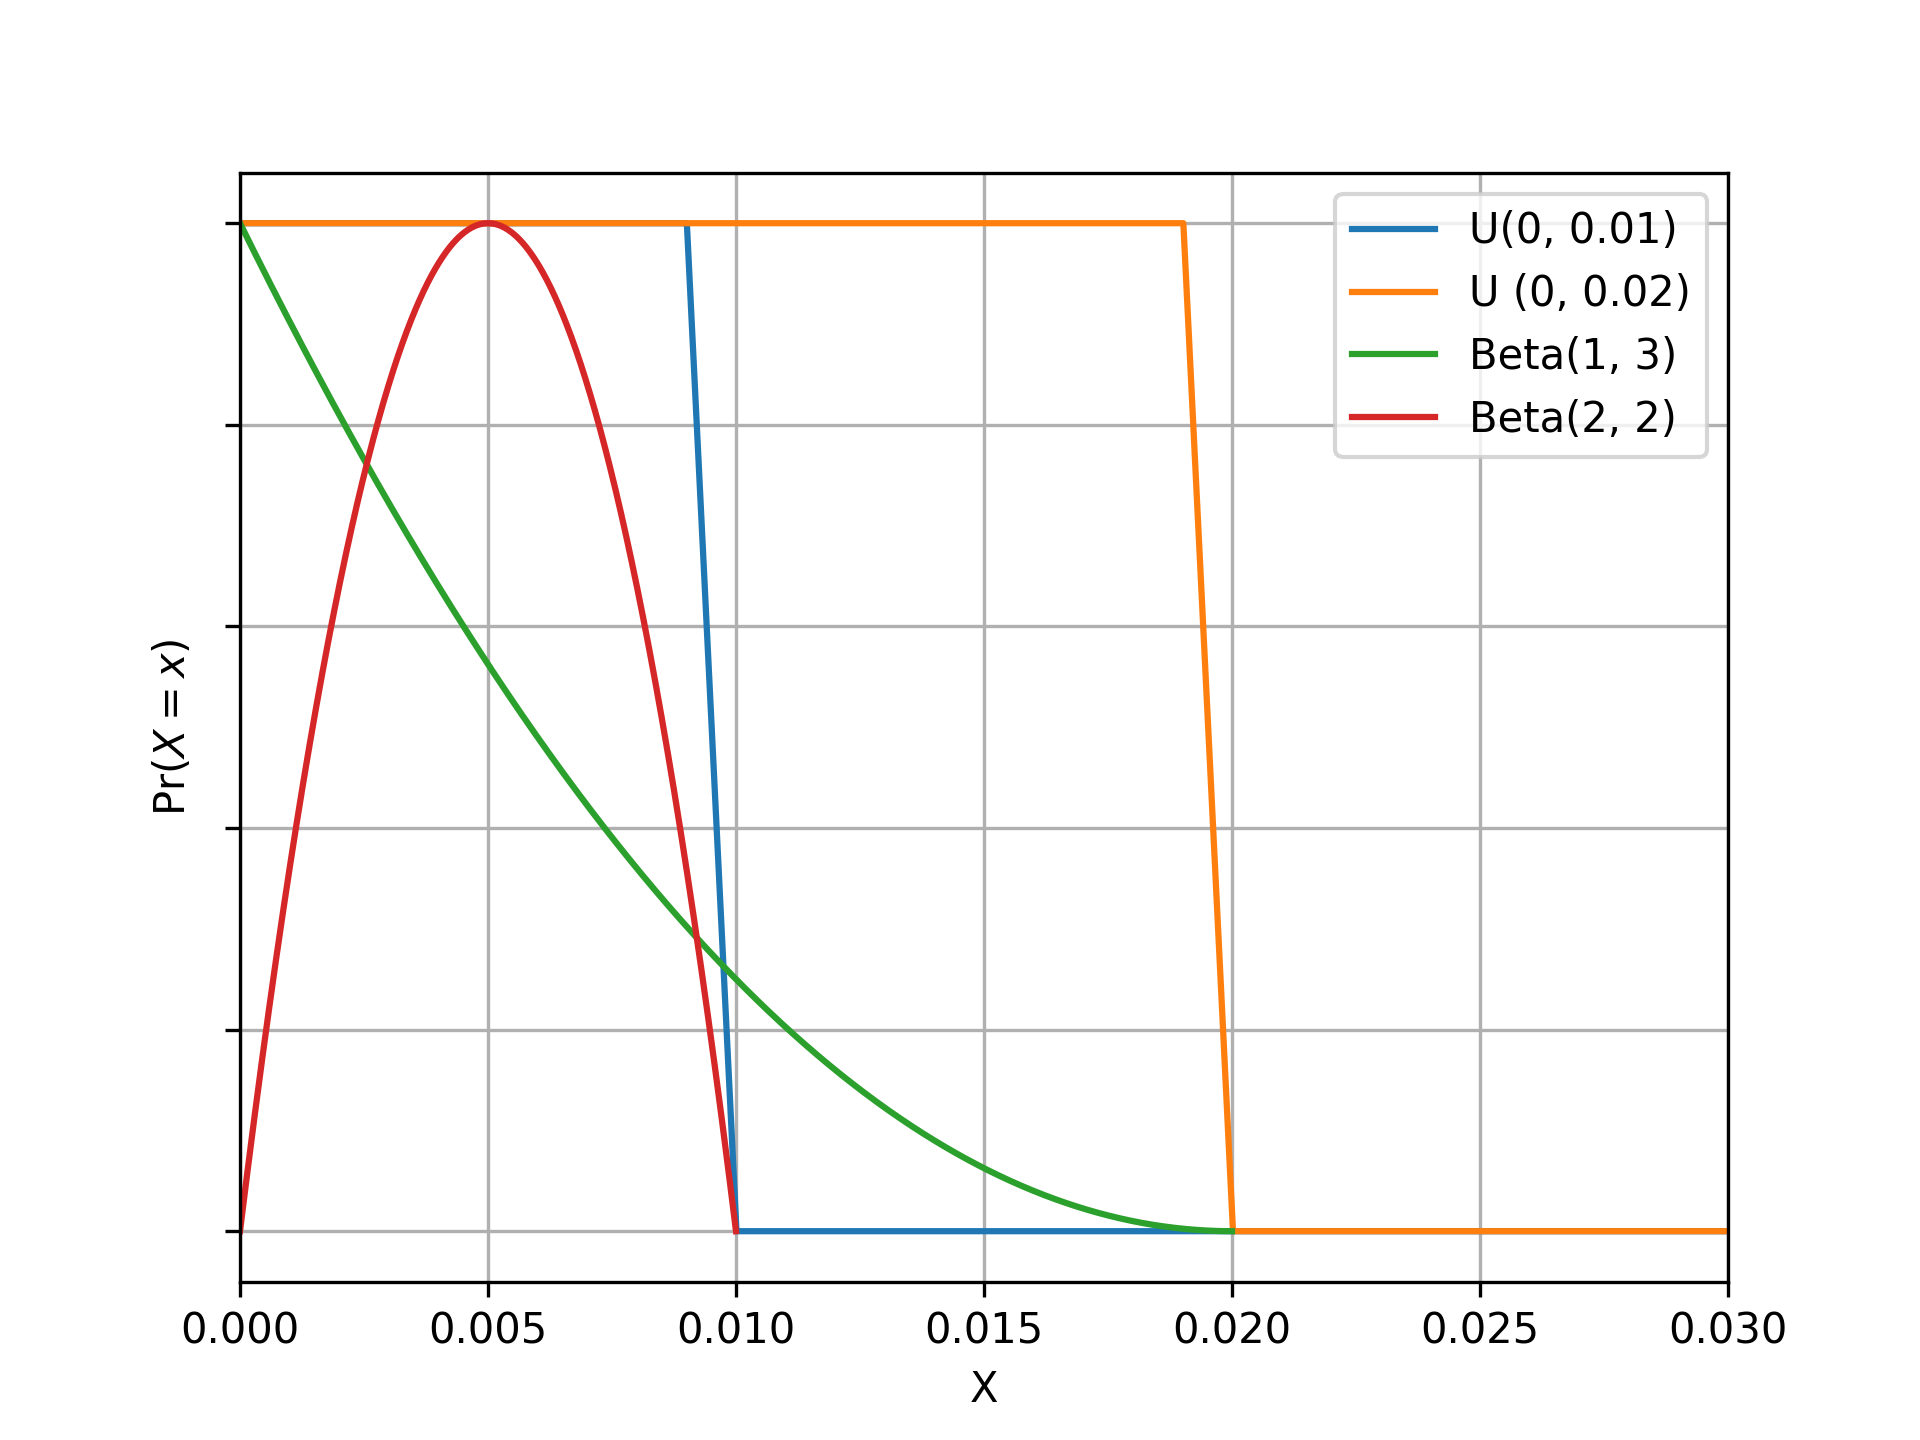
\includegraphics[width=0.5\textwidth]{probability_density_functions.png}
    \caption{Probability density functions for the four different probability distributions. We normalize the probability density functions to have a maximum value of 1 for each distribution as we are interested in the relative differences between the different distributions. While the height of the pdfs are not to scale, their shape are.}
    \label{fig:probability_density_functions}
\end{figure}


\textbf{Expected Behavior.}
Before discussing the results of the Monte-Carlo simulations in detail, let us first investigate the expected behavior of the simulations.

We have computed the expected number of times an animal is being catched at each time step. Recall that the expected values for $X_i^t$ is $0.005$ for all given distributions, except when $p\sim U(0, 0.01)$, as in that setting, the expected value rises to $0.01$.

Concretely, this means that when using $U(0, 0.01)$ as the probability to catch an animal, the number of times an animal is being catched is twice as high as when using the three other probability distribution.
Therefore, we expect the estimations of $\hat{N}$ and $\sigma_{\hat{N}}$ to be better when using $p\sim U(0, 0.01)$ as oposed to the other distributions.

Trivially, as the expected behavior of the three other distributions are identical, we expect the estimations of $\hat{N}$ and $\sigma_{\hat{N}}$ to be very identical up to the effect of the randomness introduced by the Monte-Carlo simulations.

\begin{table}[t]
    \centering 
    \caption*{$p_i \sim U(0, 0.01)$}
    \begin{tabular}{c c|c c c}
        \toprule
        & & \multicolumn{1}{|c|}{${N}=500$} & \multicolumn{1}{c|}{${N}=1000$} & \multicolumn{1}{c}{${N}=5000$} \\
        \midrule
        \multicolumn{2}{c|}{${\hat{\mathbf{N}}}$} & $590.45 \variance{311}$ & $1096.62 \variance{286}$ & $5152.14 \variance{583}$  \\
        \multicolumn{2}{c|}{\textbf{Error} (\%)} & $18.09$ & $9.66$ & $3.04$ \\
        % \hline
        \multicolumn{2}{c|}{${\hat{\mathbf{\sigma}}}_{\hat{N}}$} & $239.58 \variance{258}$ & $284.17 \variance{116}$ & $566.36 \variance{98}$\\
        % \hline
        \multirow{2}{*}{\textbf{C.I.}} & $\alpha = 0.05$ & $[299.68 \variance{85}; 1322.77 \variance{1298}]$ & $[687.34 \variance{137}; 1842.05 \variance{609}]$ & $[4179.35 \variance{423}; 6414.78 \variance{804}]$
        \\
        % 
        & $\alpha = 0.01$ & $[250.36 \variance{59}; 1740.30 \variance{2079}]$ & $[601.62 \variance{110}; 2185.30 \variance{773}]$ & $[3922.46 \variance{383}; 6884.52 \variance{890}]$ \\
        \midrule
        \multirow{2}{*}{\textbf{Coverage} (\%)} & $\alpha = 0.05$ & $94.50 \variance{22}$ & $95.70 \variance{20}$ & $94.70 \variance{22}$ \\
        & $\alpha = 0.01$ & $99.40 \variance{7}$ & $99.20 \variance{8}$ & $99.20 \variance{8}$ \\
        \multicolumn{2}{c|}{\textbf{Bias} ($\approx$)} & $8\ 181$ & $9\ 334$ & $23\ 147$ \\
        \multicolumn{2}{c|}{\textbf{Variance} ($\approx$)} & $124\ 464$ & $94\ 211$ & $330\ 364$ \\
        \multicolumn{2}{c|}{\textbf{MSE} ($\approx$)} & $132\ 646$ & $103\ 546$ & $353\ 512$ \\
        \bottomrule
    \end{tabular}
    \caption{Result from $1000$ MC simulations for estimating $\hat{N} \mid p_i \sim U(0, 0.01)$. For each value, we report on the mean (black) and standard deviation (gray). We omit the digits after the decimal point for the standard deviation for brevity.
    The Error (\%) is the absolute difference between the estimated and the true value of $N$, divided by the true value of $N$. The Bias is reported as ${\left[ \mathbb{E}[X] - X \right]}^2$.}
    \label{tab:problem_2_results_uniform_0_01}
\end{table}

\textbf{Observations.}
Let us first look at Table~\ref{tab:problem_2_results_uniform_0_01} which contains the result when using $p\sim U(0, 0.01)$.

First, it is very clear that increasing the true population size $N$ decreases the relative error of the estimator. 
Furthermore, the estimated population size $\hat{N}$ is close to the true value of $N$ for all three settings of our simulation with a deviation of approximately 90--150 animals. 

Interestingly, although the absolute error of the population estimation increases with the true number of population, the relative error of the estimated population size to the true population size decreases with increasing true population size $N$. Whereas for a small population size ($N=500$), the relative error is approximately 18\%, for larger population sizes ($N=5000$), the relative error drops to only 3\%.

The estimated standard deviation ($\hat{\sigma}_{\hat{N}} = \sqrt{\hat{\sigma}_{\hat{N}}^2}$) from the given formula perfectly matches the standard deviation computed by the Monte-Carlo simulation (refer to the gray value next to the $\hat{N}$ estimate).
Nevertheless, it is important to denote that the standard deviation of the estimated variance is very large (e.g., $\sigma_{\hat{\sigma}_{\hat{N}}} = \pm 258$ for $\hat{\sigma}_{\hat{N}} = 239.58$), hence, the estimated variance can deviate significantly across different runs. Therefore, the estimated variance is only trustworthy for large population sizes.

It is worth mentioning that although the standard deviation increases with increased population size $N$, the variance of the estimated standard deviation of the estimation of the population size decreases the larger $N$ becomes. 

We compute the coverage (percentage of times the true population size is contained in the confidence interval) for different values of $\alpha\in \{0.05, 0.01\}$ and observe that, regardless of the true population size $N$, the average coverage matches the expected coverage of the specified confidence intervals.

Interestingly, the standard deviation of the computed coverage from the Monte-Carlo simulation remains stable across all population sizes; We have a standard deviation of $\pm 22$ percentage points for $\alpha=0.05$ and $\pm 8$ percentage points for $\alpha = 0.01$.

Finally, and most interestingly, we also compute the Bias, Variance, and the Mean Squared Error (MSE) for each context of our simulations.
In Table~\ref{tab:problem_2_results_uniform_0_01}, we observe that the bias only increases slightly from $N=500 \to N=1000$ (from $90^2 \to 96^2$) but increases drastically for $N=1000 \to N=5000$, where the bias increases by $2.5$ times.

Most interestingly, the variance does not follow a simple pattern. While increasing $N=500 \to N=1000$ drops the variance by $23.7\%$ (around 30 000 units of absolute difference), when increasing the true population size from $N=1000 \to N=5000$, we observe an increase of the variance of the estimation of the population size $350\%$.

Finally, because the variance is around 1 order of magnitude larger than the bias term, the MSE follows the general trend described in the variance.

\textbf{Comparison to other Probability Distributions.}
While we went into details on the results from Table~\ref{tab:problem_2_results_uniform_0_01}, these results result from $p\sim U(0, 0.01)$ and may therefore deviate from the results for the other probability distributions.

First, as hypothesized previously, the results between 
\begin{itemize}
    \item $p \sim U(0, 0.01)$ - See Table~\ref{tab:problem_2_results_uniform_0_01}
    \item $p \sim 0.02 \cdot \mathrm{Beta}(1, 3)$ - See Table~\ref{tab:problem_2_results_beta_1_3}
    \item $p \sim 0.01 \cdot \mathrm{Beta}(2, 2)$ - See Table~\ref{tab:problem_2_results_beta_2_2}
\end{itemize}
are extremely similar.
In fact, not only are the returned values all within the standard deviation of the results from each other --- regardless of the true population size or the metric.
Naturally, as each distribution has a different probability density function, and that Monte-Carlo simulation inherently introduces some noise, the results slightly differs between Table~\ref{tab:problem_2_results_uniform_0_01}, Table~\ref{tab:problem_2_results_beta_1_3}, and Table~\ref{tab:problem_2_results_beta_2_2}.

\begin{table}[t]
    \centering 
    \caption*{$p_i \sim U(0, 0.02)$}
    \begin{tabular}{c c|c c c}
        \toprule
        & & \multicolumn{1}{|c|}{${N}=500$} & \multicolumn{1}{c|}{${N}=1000$} & \multicolumn{1}{c}{${N}=5000$} \\
        \midrule
        \multicolumn{2}{c|}{${\hat{\mathbf{N}}}$} & $527.70 \variance{98}$ & $1035.16 \variance{134}$ & $5088.17 \variance{284}$  \\
        \multicolumn{2}{c|}{\textbf{Error} (\%)} & $5.54$ & $3.52$ & $1.76$ \\
        % \hline
        \multicolumn{2}{c|}{${\hat{\mathbf{\sigma}}}_{\hat{N}}$} & $97.71 \variance{29}$ & $133.04 \variance{27}$ & $288.03 \variance{25}$\\
        % \hline
        \multirow{2}{*}{\textbf{C.I.}} & $\alpha = 0.05$ & $[381.03 \variance{57}; 774.58 \variance{172}]$ & $[818.85 \variance{91}; 1347.52 \variance{198}]$ & $[4568.45 \variance{240}; 5700.59 \variance{337}]$
        \\
        % 
        & $\alpha = 0.01$ & $[348.62 \variance{49}; 882.73 \variance{206}]$ & $[765.73 \variance{82}; 1471.85 \variance{225}]$ & $[4421.98 \variance{228}; 5914.73 \variance{356}]$ \\
        \midrule
        \multirow{2}{*}{\textbf{Coverage} (\%)} & $\alpha = 0.05$ & $95.00 \variance{21}$ & $95.30 \variance{21}$ & $94.60 \variance{22}$ \\
        & $\alpha = 0.01$ & $99.40 \variance{7}$ & $98.80 \variance{10}$ & $98.70 \variance{11}$ \\
        \multicolumn{2}{c|}{\textbf{Bias} ($\approx$)} & $767$ & $1\ 236$ & $7\ 774$ \\
        \multicolumn{2}{c|}{\textbf{Variance} ($\approx$)} & $10\ 398$ & $18\ 460$ & $83\ 612$ \\
        \multicolumn{2}{c|}{\textbf{MSE} ($\approx$)} & $11\ 166$ & $19\ 696$ & $91\ 387$ \\
        \bottomrule
    \end{tabular}
    \caption{Result from $1000$ MC simulations for estimating $\hat{N} \mid p_i \sim U(0, 0.02)$. For each value, we report on the mean (black) and standard deviation (gray). We omit the digits after the decimal point for the standard deviation for brevity.
    The Error (\%) is the absolute difference between the estimated and the true value of $N$, divided by the true value of $N$. The Bias is reported as ${\left[ \mathbb{E}[X] - X \right]}^2$.}
    \label{tab:problem_2_results_uniform_0_02}
\end{table}

However, when we look at Table~\ref{tab:problem_2_results_uniform_0_02}, which contains the results for $p\sim U(0, 0.02)$, which has a higher expected value (see Equation~\ref{eq:expectation_xi_u02}), we observe that, indeed, the values differ (significantly) from the results of the other distributions.

First, the deviation of the estimated to the true population size is significantly lower for $p\sim U(0, 0.02)$ compared to the other distributions. 
The relative error is the perfect metric to quantify the change in deviation, as it decreases from 18\% for $p\sim U(0, 0.01)$ to 5.54\% for $p\sim U(0, 0.02)$ when $N=500$, which is a decrease of $70\%$. Increasing the true population size to larger values has a similar effect. For example, for $N=5000$, the relative error drops from 3\% to 1.76\%.

We remark that the estimated standard deviation and the true standard deviation of the estimated population size are very similar for $p\sim U(0, 0.02)$ too, with a lower standard deviation compared to the other distributions.

Similarly, the coverage remains stable across all population sizes, demonstrating that the confidence intervals are well-calibrated. Note that the standard deviation of the coverage is the same as for the other distributions, indicating that the std.\ of the converage is potentially independent of the probability distribution used.

Finally, the MSE follows a different pattern as computed for the other distributions.
While the bias increases with the same pattern but lower values as the other distributions, the variance also increases linearly with the size of the true population size. 
Therefore, the MSE roughtly follows a linear increase with the size of the true population size.

However, the increase in the quality of the estimators is significant, as the MSE for $N=5000$ drops from around 350 000 units to around 90 000 units, which is a decrease of around 75\%.


\textbf{Discussion --- MSE.}
One of the most surprising observations is the change of the MSE w.r.t.\ the true population size. The results from Table~\ref{tab:problem_2_results_uniform_0_01} and Table~\ref{tab:problem_2_results_beta_2_2} show that the MSE (and variance) follows a v shape when increasing the true population size, where $N=1000$ has the lowest MSE when comparing to $N=500$ and $N=5000$.

We hypothesize that this phenomenon is simply due to the fact that the number of steps ($T=40$) is too low to obtain accurate estimations when using probability distribitions that have a low $\mathbb{E}\left[ X_i^t = 1 \right]$.
We hypothesize that doubling the number of time steps should give us similar results as the results from Table~\ref{tab:problem_2_results_uniform_0_02} with $p\sim U(0, 0.02)$.

This hypothesis is supported by the results in Table~\ref{tab:problem_2_results_uniform_0_02} where the MSE follows a linear increase w.r.t.\ $N$.

To verify our hypothesis, we run the simulation using $p\sim U(0, 0.01)$ for twice as long, namely $T=80$ instead of 40 time steps. We report on the results in Table~\ref{tab:problem_2_results_extra_long} in the Appendix.
In short, we observe that the results from Table~\ref{tab:problem_2_results_extra_long} matches the results obtained in Table~\ref{tab:problem_2_results_uniform_0_02}, therefore validating our hypthesis.

\textbf{Discussion --- Estimated Population Size.}
Interestingly, the estimated population size reported by our Monte-Carlo simulations always over-estimate the true population size. 
We want to understand this better, and understand whether this is a systematic property of the given estimator.

First, we hypothesize that most of the variance is due to the estimation of $\hat{f_0}$. As the given formula for estimating $\hat{f_0}$ is dependent on whether $f_2 \neq 0$ or $f_2 = 0$, we aim to first understand how similar both formulas are.
To this end, we plot in Figure~\ref{fig:f0_hat_comparison} the estimated $\hat{N}$ over 100 time steps for a single run of the Monte-Carlo simulation with true population size $N=1000$ and $p\sim U(0, 0.01)$.

In Figure~\ref{fig:f0_hat_comparison}, we clearly observe that, whenever $f_2 = 0 \to f_2 > 0$, the estimation of $\hat{f_0}$ is not continuous in time and drasticaly drops. Interestingly, as soon as $f_2 > 0$, the estimator of $\hat{N}$ seems to approach the true population size. 

We also plot the true value for $f_0$ and the estimated value for $\hat{f_0}$ over the same number of time steps in Figure~\ref{fig:f0_hat_comparison}. 
We can clearly see that the estimated values for $\hat{f_0}$ approach the true value for $f_0$ over time.

\begin{figure}[t]
    \centering
    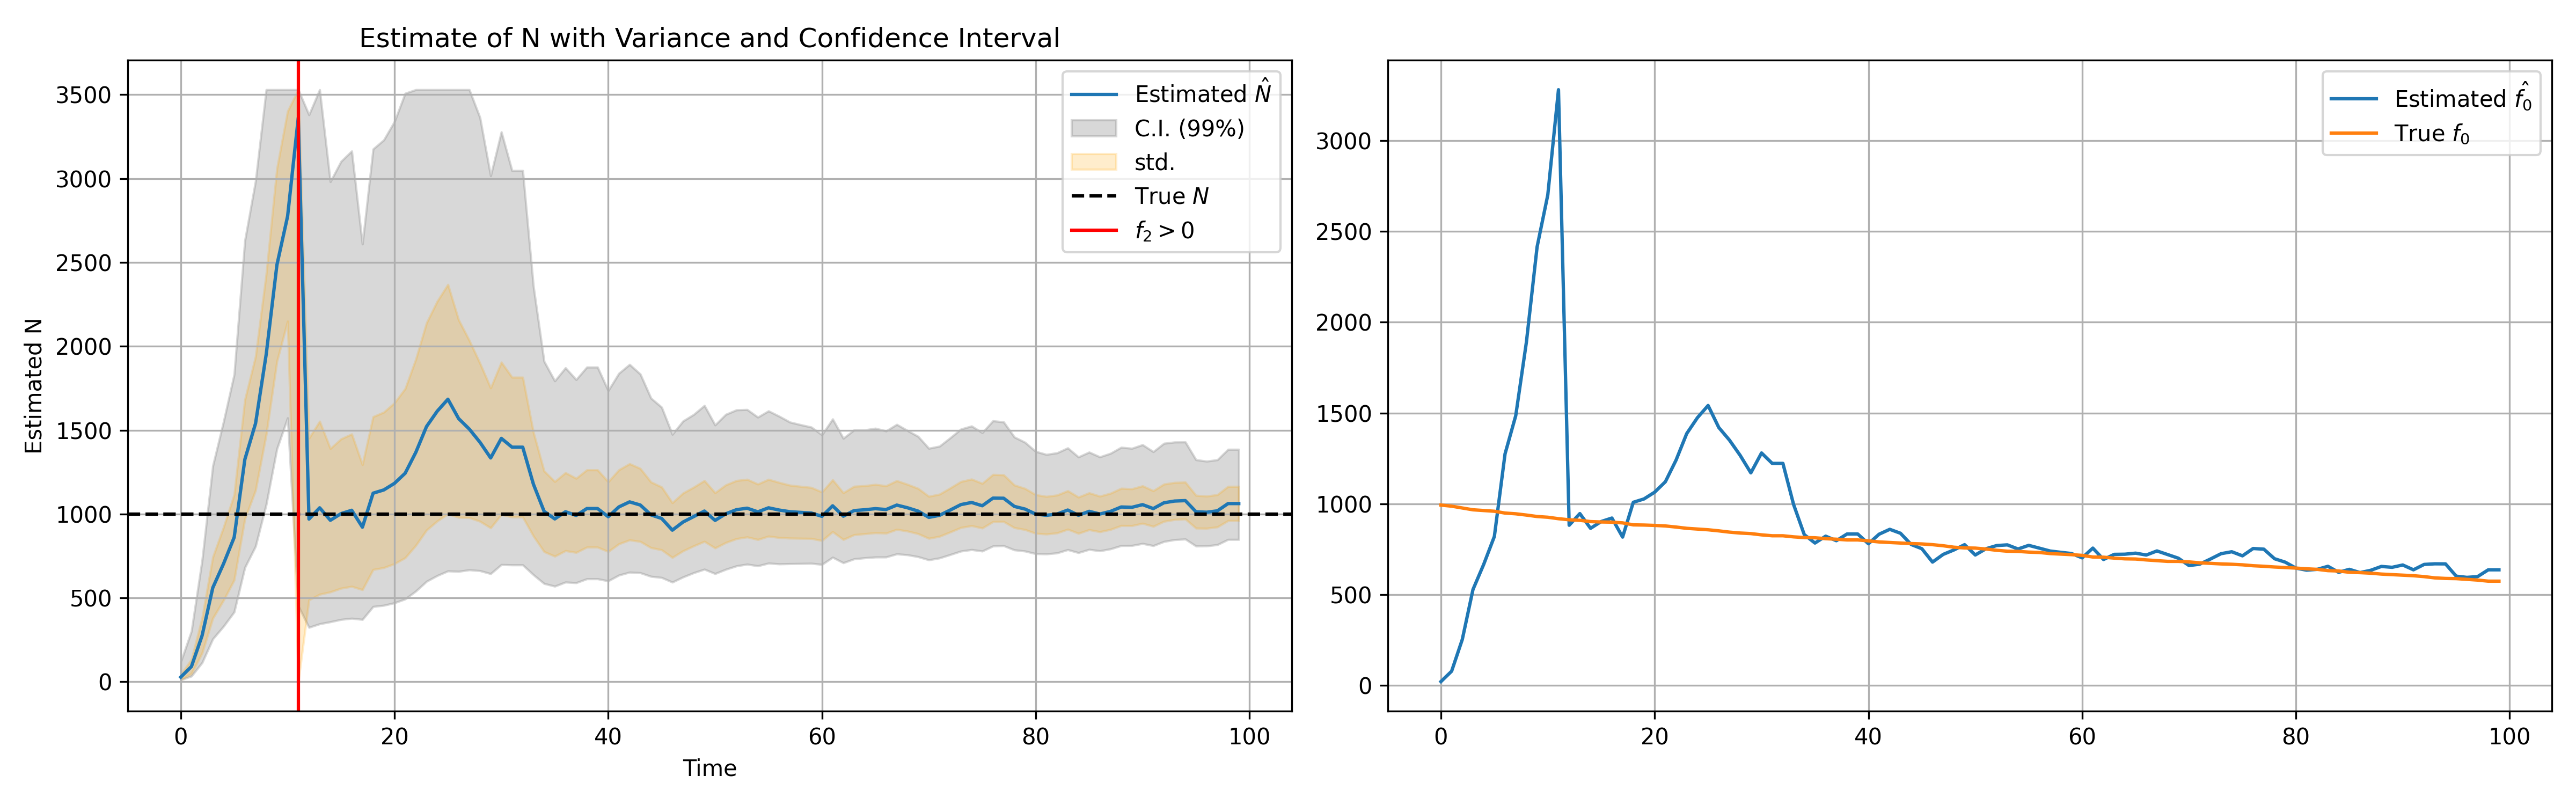
\includegraphics[width=\textwidth]{single_run.png}
    \caption{Single run of the Monte-Carlo simulation for estimating $\hat{N}$ with a true population size of $N=1000$ and a probability distribution of $p_i \sim U(0, 0.01)$.}
    \label{fig:f0_hat_comparison}
\end{figure}



We remark that the behavior observed in Figure~\ref{fig:f0_hat_comparison} is not systematic, as the jump is very extreme. We found this example by chance when plotting the results for a single run. However, it provides us with great insights into the behavior of the estimators.

\begin{center}
    \noindent\rule{0.2\linewidth}{0.4pt}
    \hspace{0.02\linewidth}
    \textbf{End of the core answer of Question 2}
    \hspace{0.02\linewidth}
    \rule{0.2\linewidth}{0.4pt}
\end{center}

While this remaining part relates to the discussion of Problem 2, and can therefore be considered as part of the answer, we understand that only readers interested in the problem formulated in Equation~\ref{eq:goal_equation} will be interested in this section. 
Therefore, if the reader thinks that the explanation stated above is sufficient, we do not force them to read the remaining part.

\textbf{Analytical Analysis --- Over-Estimation of the Population Size.}

In the remaining part of this section, we will investigate analytically whether the over-estimation of the population size is a systematic property of the given estimator.


Formally, we are interested in the following question
\begin{equation}
    \Pr(\hat{N} > N) > \Pr(\hat{N} \leq N)\;.
    \label{eq:goal_equation}
\end{equation}

To this end, we will assume that the estimator is unbiased, i.e., that $\mathbb{E}[\hat{N}] = N$. 
Note that Equation~\ref{eq:goal_equation} is not in contradiction with the unbiasness of the estimator, as the expected value is the value towards which the estimator converges to in the limit of the number of samples. However, for finite samples, even if the estimator has a theoretical mean of $N$, if the distribution of the estimated population size is skewed, it is possible that Equation~\ref{eq:goal_equation} holds. 

% Whether this is the case is beyond the scope of this assignment. Investigating this could be an interesting future work.

Before we start, let us first formally define some notation and defintions of $f_i$ that allows us to derive the probability for $\hat{N} > N$.

Let us denote an animal as $X_i$ with $i\in \{1, \dots, N\}$ and $X_i^t\in \{0, 1\}$ denoting whether the animal $i$ has been caught at time step $t$.
Therefore, we can define 
\begin{equation*}
    X_i = \sum_{t=1}^T X_i^t\;,
\end{equation*}
i.e., the total number of times the animal has been caught after $T$ time steps.

Logically, we have that $X_i^t \sim \mathrm{Bernoulli}(p)$ with $p$ being the probability of being caught at time step $t$. In our setting, $p$ follows a specified probability distribution.

We have that $X_i^t$ are i.i.d.\ w.r.t.\ the time steps $t$ and the animals $i$. These are important assumptions.
From this, it follows that $X_i \sim \mathrm{Binomial}(T, p)$ as we have a sum of $T$ independent Bernoulli variables.

We can now formally define $f_k$ as follows using the following set 
\begin{equation*}
    S_k = \left\{ X_i : i \in \{1, \dots, N\} \mid X_i = k \right\}
\end{equation*}
which contains all the animals that have been caught exactly $k$ times within the $T$ time steps.
Therefore, $f_k$ can be defined as follows:
\begin{equation*}
    f_k = |S_k|\;.
\end{equation*}

Because $f_k$ is a random variable, we can define the probability distribution of $f_k$ w.r.t.\ the number of time steps $t$ as binomial distribution:
\begin{align*}
    \Pr(f_k = n\mid T=t) = \mathrm{Binomial}(N, n, \Pr(X_i = k\mid T=t))\;. \quad n \in \{0, 1, \dots, N\}
\end{align*}

Therefore, we need to compute the probability of an animal being caught exactly $k$ times within the $T$ time steps. We have
\begin{align*}
    \Pr(X_i = k \mid T=t') = \mathrm{Binomial}(t', k, \Pr(X_i^t = 1))
\end{align*}
where $\Pr(X_i^t = 1)$ is the probability of an animal being caught at time step $t$.
Because $X_i^t$ is a binary variable, its expected value is its probability, and we can therefore re-use the expected values for the different given probabilities that we computed earlier (see Equation~\ref{eq:expectation_xi_u01},~\ref{eq:expectation_xi_u02},~\ref{eq:expectation_xi_beta13},~\ref{eq:expectation_xi_beta22}).

% We derive the following proposition, which we will use later. Note that Equation~\ref{} is entirely derived by ChatGPT as I was searching whether there were known results for this property. I could have easily derived it myself, however, I wanted to be sure that it lead somewhere. Note that I added some intermediate steps such that I understand each step fully:
% \begin{align*}
%     n \cdot \binom{N}{n} &= n \frac{N!}{n!(N-n)!} \\
%     &= \frac{N!}{(n-1)!(N - n)!} \\
%     &= N\frac{(N-1)!}{(n-1)!(N-n)!} \\
%     % &= N\frac{(N-1)!}{(n-1)!(N-n-1)!\cdot(N-n)} \stepandtag \label{eq:binomial_property} \\
%     % &= N \frac{(N-1)!}{(n-1)!((N-1)-(n-1))!}
%     % &= N \frac{(N-1)!}{(n-1)!(N-n)!} \\
%     &= N \frac{(N-1)!}{(n-1)!(N-1-n+1)!} \\
%     &= N \frac{(N-1)!}{(n-1)!((N-1)-(n-1))!} \\
%     &= N \binom{N-1}{n-1}
% \end{align*}

We can now compute the expected value for each $f_k$:
{
\allowdisplaybreaks
\begin{align*}
    \mathbb{E}\left[ f_k \mid T=t \right] &= \sum_{n=0}^N n \cdot \Pr(f_k = n \mid T=t) \\
    &= \sum_{n=1}^N n \cdot \mathrm{Binomial}(N, n, \Pr(X_i = k \mid T=t)) \\
    &= \sum_{n=1}^N n \cdot \mathrm{Binomial}(N, n, \mathrm{Binomial}(t, k, p)) 
    % &&p = \mathbb{E}[X_i^t = 1]
    \\
    &= \sum_{n=1}^N n \cdot \mathrm{Binomial}\left( N, n, \binom{t}{k} p^k {(1-p)}^{t-k} \right) \\
    &= \mathbb{E}\left[ \mathrm{Binomial} \left( N, n, \binom{t}{k} p^k {(1-p)}^{t-k} \right) \right] \\
    &= N \cdot \binom{t}{k} p^k {(1-p)}^{t-k}
\end{align*}
}
% We can simplify this further by using the Binomial theorem (also known as Binomial expension).\!\footnote{See \url{https://en.wikipedia.org/wiki/Binomial_theorem}. The idea of using it came from ChatGPT, as I was searching for ways to simplify the expression with the complex power.}

Therefore, we can now compute the expected value for $n$:
\begin{align*}
    \mathbb{E}\left[ n \right] &= \mathbb{E}\left[ \sum_{t=1}^T f_k \right] \\
    &= \sum_{k=1}^T \mathbb{E}\left[ f_k \right] \\
    &= \sum_{k=1}^T \mathbb{E}\left[ f_k \mid T=T\right] \\
    % &= \sum_{k=1}^T \mathbb{E}\left[ f_k \mid T=T\right] \\
    &= \sum_{k=1}^T N \cdot \binom{t}{k} p^k {(1-p)}^{T-k} \\
    &= N \cdot \sum_{k=1}^T \binom{t}{k} p^k {(1-p)}^{T-k} \\
    &= N \cdot \left[ \left( \sum_{k=0}^T \binom{t}{k} p^k {(1-p)}^{T-k} \right) - \binom{t}{0} p^0 {(1-p)}^{T-0}  \right] \\
    &= N \cdot \left[ 1 - 1{(1-p)}^{T} \right]  \\
    &= N \cdot \left( 1 - {(1-p)}^T \right) \stepandtag \label{eq:expected_value_n}\;.
\end{align*}
We report on the expected values for $n$ with $T=40$ for our four probability distributions in Table~\ref{tab:expected_value_n}.
\begin{table}[t]
    \centering
    \begin{tabular}{c|c c c}
        \toprule
         & \multicolumn{3}{c}{Expected Value for $n$} \\
        \midrule
        $N$ & $500$ & $1000$ & $5000$ \\
        \midrule
        $U(0, 0.01)$ & $90.83$ & $181.67$ & $908.39$\\
        $U(0, 0.02)$ & $165.51$ & $331.02$ & $1655.14$\\
    \end{tabular}
    \caption{Expected value for $n$ for $T=40$ and $N \in \{500, 1000, 5000\}$ for the different probability distributions.}
    \label{tab:expected_value_n}
\end{table}
Note that Equation~\ref{eq:expected_value_n} is equal to 
\begin{align*}
    \mathbb{E}\left[ n \right] &= N \cdot \left( 1 - {(1-p)}^T \right) \\
    &= N \cdot \left( 1 - \binom{T}{0} p^0 (1-p)^T \right) \\
    &= N - N \cdot \binom{T}{0} p^0 (1-p)^T \\
    &= N - \mathbb{E}\left[ f_0 \mid T=T \right] 
\end{align*}
which is exactly what we would expect.
% Let us now compute the skewness of the distribution of $n$. 
% Because we know that $f_k$ follows a binomial distribution, we can compute 

Because $\hat{N} = n + \hat{f_0}$, we now compute the expected value for $\hat{f_0}$.
As $\hat{f_0}$ is conditional on whether $f_2 \neq 0$ or $f_2 = 0$, we need to compute the probability of $f_2 = 0$ and $f_2 \neq 0$.
% Note that we assume that $f_2 \neq 0$, as otherwise we would need to marginalize over the probability of $f_2 = 0$. Given that we have $T \gg 0$, we expect the probability of $f_2 = 0$ to be extremely small, and therefore negligable.
% Nevertheless, we can easily compute the probability of $f_2 = 0$:
Because we model $f_k$ as a binomial distribution, we can easily compute the probability of $\Pr(f_2 = 0)$. We have 
\begin{align*}
    \Pr(f_2 = 0 \mid T=T) &= \mathrm{Binomial}(N, 0, \Pr(X_i = 2\mid T=T)) \\
    &= (1 - \Pr(X_i = 2\mid T=T))^N \\
    &= {\left( 1 - \mathrm{Binomial}(T, 2, p) \right)}^N\;.
\end{align*}
We report on the probabilities for our four probability distributions for $p$ in Table~\ref{tab:probability_f2_eq_0}. We also plot the probability changing over time in Figure~\ref{fig:probability_f2_eq_0_over_time}.

\begin{table}[t]
    \centering
    \begin{tabular}{c|c c c}
        \toprule
         & \multicolumn{3}{c}{$\Pr(f_2 = 0 \mid T=40)$} \\
        \midrule
        $N$ & $500$ & $1000$ & $5000$ \\
        \midrule
        $p=0.01$ & $1.3 \times 10^{-12}$ & $1.7 \times 10^{-24}$ & $1.6 \times 10^{-119}$ \\
        $p=0.005$ & $2.96 \times 10^{-4}$ & $8.77 \times 10^{-8}$ & $5.19 \times 10^{-36}$ \\
        % \bottomrule
    \end{tabular}
    \caption{Probability for $f_2 = 0$ $n$ for $T=40$ and $N \in \{500, 1000, 5000\}$ for the different probability distributions.}
    \label{tab:probability_f2_eq_0}
\end{table}




Before investigating the case where $f_2\neq 0$, let us first investigate the bias of $\hat{f_0}\mid f_2 = 0$.
We have 
{
\allowdisplaybreaks
\begin{align*}
    \mathbb{E}\left[ \hat{f_0} \mid f_2 = 0, T=t \right] &= \mathbb{E}\left[ \frac{f_1^2 - f_1}{2} \right] \\ 
    &= \sum_{n=0}^N \frac{n^2 - n}{2} \cdot \Pr(f_1 = n \mid T=t) \\
    &= \sum_{n=0}^N \frac{n^2 - n}{2} \cdot \mathrm{Binomial}(N, n, \Pr(X_i = 1 \mid T=t)) \\
    &= \sum_{n=0}^N \frac{n^2 - n}{2} \cdot \mathrm{Binomial}(N, n, \mathrm{Binomial}(t, 1, p)) \\
    &= \sum_{n=0}^N \frac{n^2 - n}{2} \cdot \mathrm{Binomial}(N, n, \binom{t}{1} p^1 {(1-p)}^{t-1})
    % &= \sum_{n=0}^N \frac{n^2 - n}{2} \cdot \binom{N}{n} {\left( \binom{t}{1} p^1 {(1-p)}^{t-1} \right)}^{n} {\left( 1 - \binom{t}{1} p^1 {(1-p)}^{t-1} \right)}^{N-n} \\
    % &= \sum_{n=0}^N \frac{n^2 - n}{2} \cdot \binom{N}{n} {\binom{t}{1}}^n p^n {(1-p)}^{(t-1)\cdot n} {\left( 1 - \binom{t}{1} p^1 {(1-p)}^{t-1} \right)}^{N-n} \\
\end{align*}
which we we cannot simplify further (at least such that is gives us more insights). We use python to compute the expected value for $\hat{f_0} \mid f_2 = 0, T=40$ for our four probability distributions and report on the results in Table~\ref{tab:expected_value_f0_f2_eq_0}. While the expected values for $\hat{f_0}\mid f_2 = 0$ are very large, it is easy to see that when multiplied with the probability of $f_2 = 0$, we would get values that are almost zero. The interested reader can find a plot describing the rescaled expected value in Figure~\ref{fig:expectation_f0_f2_eq_0_rescaled} in the Appendix.


\begin{table}[t]
    \centering
    \begin{tabular}{c|c c c}
        \toprule
         & \multicolumn{3}{c}{$\mathbb{E}[\hat{f_0} \mid f_2 = 0, T=40]$} \\
        \midrule
        $N$ & $500$ & $1000$ & $5000$ \\
        \midrule
        $p=0.01$  & $9113.93$   & $36492.25$  & $913036.85$ \\
        $p=0.005$ & $3375.21$   & $13514.37$  & $338129.79$ \\
        % \bottomrule
    \end{tabular}
    \caption{Expected value for $\hat{f_0}$ conditioned on $f_2 = 0$ for $T=40$ and $N \in \{500, 1000, 5000\}$ for different values of $p$.}
    \label{tab:expected_value_f0_f2_eq_0}
\end{table}
}

Let us now investigate the bias of $\hat{f_0}$ when $f_2 \neq 0$. As $\hat{f_0}$ is defined as a function of $f_1$ and $f_2$, and that both of them are dependent,\!\footnote{We attach in the Appendix (See Section~\ref{sec:proof_dependency_f1_f2}) a proof of the dependency of $f_1$ and $f_2$ generated by ChatGPT.  As the proof is not critical for the continuation of this derivation, we add it to the Appendix for the interested reader. Note that while we have deleted the exact output of ChatGPT, the idea of this proof is still to be credited to ChatGPT.} we have to model their probability jointly for a fully analytical derivation.
While it is very tempting to add a independence assumption on the distributions of $f_1$ and $f_2$, their correlation is too strong to be ignored, and the obtained results are not meaningful.\!\footnote{This was our first attempt. However, our formula estimated $\mathbb{E}[\hat{f_0}\mid f_2 > 0, T=40]$ to be almost zero for all probability distributions and sample sizes.}
% However, as modeling the joint probability is very complex, we resort to an approximation by introducing an assumption that doesn't hold.
% Therefore, for ease of computability, we will assume that $f_1$ and $f_2$ are independent. Note that their correlation is not zero, and can be meaningful for larger catching probabilities $p$. 
We show the correlations for our probability distributions in Table~\ref{tab:correlation_f1_f2} in the Appendix.

% We can now compute the expected value of $\hat{f_0}\mid f_2 > 0$ as follows:
% {
% \allowdisplaybreaks
% \begin{align*}
%     \mathbb{E}[\hat{f_0}\mid f_2 > 0] &= \mathbb{E}\left[ \frac{f_1^2}{2 f_2} \mid f_2 > 0 \right] \\
%     &= \sum_{n=0}^{N-1} \sum_{m=1}^{N-n} \frac{n^2}{2 m} \cdot \Pr(f_1 = n \mid T=t) \cdot \Pr(f_2 = m \mid T=t) \stepandtag \label{eq:expectation_f0_f2_gt_0}
%     % &= \sum_{n=0}^{N-1} \sum_{m=1}^{N-n} \frac{n^2}{2 m} \cdot \Pr(f_1 = n \mid T=t) \cdot \Pr(f_2 = m \mid T=t) \stepandtag \label{eq:expectation_f0_f2_gt_0}
%     % &= \sum_{n=0}^{N-1} \sum_{m=1}^{N-n} \frac{n^2}{2 m} \cdot \Pr(f_1 = n \mid T=t) \cdot \Pr(f_2 = m \mid T=t) \\
% \end{align*}
% which we could simplify further, however, we believe that we would not gain a relationship to $f_0$ by doing so. Therefore, we resort to modeling the expectation from Equation~\ref{eq:expectation_f0_f2_gt_0} using Python. 
% }

The only way to compute $\mathbb{E}[\hat{f_0}\mid f_2 > 0]$ is by marginalizing over all possible values for all $f_i$ with $f_i \notin \{1, 2\}$, i.e.,
\begin{align*}
    \mathbb{E}[\hat{f_0}\mid f_2 > 0] &= \mathbb{E}\left[ \frac{f_1^2}{2 f_2} \mid f_2 > 0 \right] \\
    &= \sum_{n=0}^{N-1} \sum_{m=1}^{N-n} \frac{n^2}{2 m} \cdot \Pr(f_1 = n, f_2 = m \mid T=t) \\
    &= \sum_{n=0}^{N-1} \sum_{m=1}^{N-n} \frac{n^2}{2 m} \cdot \left( \sum_{k_3 = 0}^{N-n-m} \cdots \sum_{k_N = 0}^{N-n-m-\sum_{i=3}^{N}k_i} \Pr(f_1 = n, f_2 = m, f_3 = k_3, \dots, f_N=k_N \mid T=t) \right) \stepandtag \label{eq:expectation_f0_f2_gt_0_marginalized}
\end{align*}
which is computationally infeasible. Furthermore, we cannot simplify Equation~\ref{eq:expectation_f0_f2_gt_0_marginalized} , as every $f_i$ is dependent on each $f_j$ with $i\neq j$. Note that especially for our simulation size, using $N=5000$ would result in a value proportional to $2^{5000}$, which is a number with 1506 digits.

Therefore, without further assumptions, we are unsure whether we can show that $N$ is unbiased --- let alone skewed --- in a fully analytical way.

Nevertheless, as we can model individual $f_i$ using a binomial distribution, we can model the skewness of both $f_1$ and $f_2$ analytically. This might give us some insights into whether Equation~\ref{eq:goal_equation} holds.


\textbf{Skewness}

Let us now investigate the skewness of $f_i \sim \mathrm{Binomial}(T, p_i)$. 
It is a well known fact that the skewness of a binomial distribution is given by 
\begin{equation*}
    \mathrm{Skewness}(f_i) = \frac{(1-p) - p}{\sqrt{N \cdot p \cdot (1-p)}}\;.
\end{equation*}

For $f_1$, we have that 
\begin{align*}
    \mathrm{Skewness}(f_1) &= \frac{(1 - \Pr(X_i = 1 \mid T=T)) - \Pr(X_i = 1 \mid T=T)}{\sqrt{N \cdot \Pr(X_i = 1 \mid T=T) \cdot (1 - \Pr(X_i = 1 \mid T=T))}} \\
    &= \frac{\left( 1 - \binom{T}{1} p^1 {(1-p)}^{T-1} \right) - \binom{T}{1} p^1 {(1-p)}^{T-1}}{\sqrt{
        N \cdot \left( 1 - \binom{T}{1} p^1 {(1-p)}^{T-1} \right) \cdot \binom{T}{1} p^1 {(1-p)}^{T-1}
    }} \\
    &= \frac{ 1 - 2 \cdot \binom{T}{1} p^1 {(1-p)}^{T-1}}{\sqrt{
        N \cdot \left( 1 - \binom{T}{1} p^1 {(1-p)}^{T-1} \right) \cdot \binom{T}{1} p^1 {(1-p)}^{T-1}
    }} 
\end{align*}
which we will compute using python. This results in the results shown in Table~\ref{tab:skewness_f1_f2}.


\begin{table}[tbp]
    \centering
    \begin{tabular}{c|c c c| c c c}
        \toprule
         & \multicolumn{3}{c}{$\mathrm{Skewness}(f_1)$} & \multicolumn{3}{c}{$\mathrm{Skewness}(f_2)$} \\
        \midrule
        $N$ & $500$ & $1000$ & $5000$ & $500$ & $1000$ & $5000$ \\
        \midrule
        $p=0.01$  & $0.0463$   & $0.0327$  & $0.0146$ & $0.17799$ & $0.12585$ & $0.05628$ \\
        $p=0.005$ & $0.0809$   & $0.0572$  & $0.0256$ & $0.34368$ & $0.24302$ & $0.10868$ \\
        % \bottomrule
    \end{tabular}
    \caption{Skewness for $f_1$ and $f_2$ for $T=40$ when modeled as a binomial distribution.}
    \label{tab:skewness_f1_f2}
\end{table}

Recall that a positive value for skewness indicates that the distribution has a median and mode on the left of the mean, and therefore the majority of the values are on the left, and the distribution is tailed to the right. A negative value has the same interpretation, but flipped. We added a visualization of the interpretation of the value of skewness in Figure~\ref{fig:interpretation_skewness} in the Appendix.

From Table~\ref{tab:skewness_f1_f2}, it is easy to see that all values are positive. Therefore, we know that $f_1$ and $f_2$ have the majority of their values to the left of the mean, i.e., have a lower value than the mean.
Naturally, the more samples we have, the less skewed the distribution is, this is also reflected in the table.

We are unable to compute the skewness of $n$, which follows the same argument as above, namely that all the $f_i$ are dependent on each other. While all the $f_i$ can be modeled using a multinomial distribution, a closed form solution to the skewness of a multinomial distribution is unknown to us, we couldn't find any literature on the topic.
% This could be an interesting topic for future research --- assuming that it is even possible.
Therefore, we assume that $n$ is either not skewed, or very lightly skewed in the oposite direction of $\hat{f_0}$. Otherwise, our argument does not hold.

However, and this is very interesting, we can say something about the skewness of $\hat{f_0}$.
When looking at the skewness of $\hat{f_0}$ in Table~\ref{tab:skewness_f1_f2}, we see that $f_1$ is less skewed than $f_2$. In fact, $f_2$ is skewed around 4--5 times more than $f_1$.
This is a very important and interesting observation. 

This shows that, for small and finite samples, we are more likely to sample values for $f_1$ and $f_2$ below the mean than above. The inequality in the skewness from Table~\ref{tab:skewness_f1_f2} indicates that, $f_2$ is sampled more below the expected value of $f_2$ than compared to $f_1$.

As we divide the less undersampled value by the more undersampled value, we argue that $\hat{f_0}$ is negatively skewed. This follows from the argument that, assuming that $\mathbb{E}[\hat{f_0}] = f_0$ holds, we would $\frac{f_1}{f_2} \approx 5$, which would mean that we overestimate $f_0$.\!\footnote{We have not used skewness in any work before. Therefore, we are unsure if this is correct. However, that this ration is larger than 1 is what we are trying to argue.}
As we are squaring the $f_1$ value, and only increasing the value of $f_2$ linearly in $\hat{f_0}$, we believe that this reduces the extremeness of the skewness of $\hat{f_0}$ significantly.

Therefore, assuming that $\mathbb{E}\left[ \hat{f_0} \right] = f_0$ holds, we argue that Equation~\ref{eq:goal_equation} holds.
How to prove this formally is unknown to us; We believe that this statement is not true in general --- as in the limit, the skewness, variance, and bias becomes zero --- but we argue that especially for small finite samples, the statement holds.

We tried to get some help from ChatGPT, as we hope that it can uncover some theorems unknown to us. While it gave us a negative answer on whether the statement holds, it said that if if our distribution is log-concave, then $P(X < E[X]) \geq \frac{1}{2}$ holds for some random variable $X \sim G$ with $G$ being a log-concave positively skewed distribution.
As the Binomial distribution is log-concave,\!\footnote{See \url{https://en.wikipedia.org/wiki/Logarithmically_concave_function}. We are unsure if this is correct for all cases, especially ours.}, we \textit{could} argue that because we hypothesize that $\frac{f_1^2}{2f_2}$ is negatively skewed, we have $P(\hat{f_0} > f_0) \geq \frac{1}{2}\Rightarrow P(\hat{f_0} > f_0) > P(\hat{f_0} \leq f_0)$. But as we are unsure about the correctness of our argument, we will only mention it here.

% This unequality in the skewness means that, when sampling for values of $f_1$ during our simulations, we are 